\subsection{Gorenstein rings}

DEFINITION 1.--- A ring A is said to be a Gorenstein ring if it is Noetherian and the \(\mathrm{A}_{\mathfrak{m}}\) -module \(\mathrm{A}_{\mathfrak{m}}\) has finite injective dimension for every maximal ideal \(\mathfrak{m}\) of A.

For a local Noetherian ring A to be a Gorenstein ring, it is necessary and sufficient that \(\mathrm{di}_{\mathrm{A}}(\mathrm{A})\) be finite; for a Noetherian ring A to be a Gorenstein ring, it is necessary and sufficient that this be so for \(\Lambda_{m}\) for every maximal ideal m of A.

PROPOSITION 10.- Let A be a Gorenstein ring; then A is a Macaulay ring, and satisfies \(\mathrm{di}_{\Lambda}(\mathrm{A}) = \dim(\mathrm{A})\) .

For every maximal ideal m of A, one has

\[
\begin{array}{l l} \dim (A _ {m}) & \leqslant \mathrm{di} _ {A _ {m}} (A _ {m}) \\ \mathrm{di} _ {A _ {m}} (A _ {m}) & = \operatorname{prof} (A _ {m}) \\ \operatorname{prof} (A _ {m}) & \leqslant \dim (A _ {m}) \end{array} \quad \begin{array}{l l} & (n ^ {\circ} 6, \text { prop. } 8) \\ & (n ^ {\circ} 6, \text { prop. } 9) \\ & (\S 1, n ^ {\circ} 4, \text { cor. } 2 \text { du   th. } 2); \end{array}
\]

whence it follows that A is a Macaulay ring, and that \(\mathrm{di}_{\mathrm{A}}(\mathrm{A}) = \dim(\mathrm{A})\) by passing to the supremum (no. 2, prop. 3).

Thus the Noetherian rings A such that \(\mathrm{di}_{\mathrm{A}}(\mathrm{A})\) is finite are the Gorenstein rings of finite dimension (prop. 3 of no. 2), and the Noetherian rings such that the A-module A is injective are the Artinian Gorenstein rings.

Examples. 1) For every multiplicative set S of a Gorenstein ring A, the ring of fractions \(S^{-1}A\) is a Gorenstein ring: indeed, let q be a maximal ideal of \(S^{-1}A\) ; it is of the form \(S^{-1}p\) , where p is a prime ideal of A not meeting S. Let m be a maximal ideal of A containing p; then the ring \(B = (S^{-1}A)_q\) is isomorphic to \(A_p\) (II, § 2, no. 5, prop. 11), hence to a ring of fractions of \(A_m\) , and consequently satisfies \(\text{di}_B(B) < +\infty\) (no. 2, cor. 1 of prop. 3).

\begin{enumerate}
\def\labelenumi{\arabic{enumi})}
\setcounter{enumi}{1}
\item
  Let A be a Gorenstein ring and let J be an ideal of A, generated by an A-regular sequence x. The quotient ring A/J is a Gorenstein ring: indeed, for every maximal ideal m of A containing J, the image in \(A_{m}\) of the sequence x is \(A_{m}\) -regular and generates the ideal \(J_{m}\) , so that \(A_{m}/J_{m}\) is a Gorenstein ring by the cor. of prop. 7 (no. 4).
\item
  Let A be a local Noetherian ring, J an ideal of A generated by an A-regular sequence of elements of \(\mathfrak{m}_{\mathrm{A}}\) . If A/J is a Gorenstein ring, then so is A (no. 4, cor. of prop. 7).
\item
  Let A be a regular local Noetherian ring; then A is a Gorenstein ring. Indeed, let x be a system of coordinates of A (VIII, § 5, no. 1, def. 1). The sequence x is A-regular (loc. cit., no. 2, th. 1) and generates the ideal m\_A; one can therefore apply example 3.
\item
  Every quotient ring of a principal ideal ring is a Gorenstein ring (example 2). In particular, every monogenic algebra over a field is a Gorenstein ring.
\end{enumerate}

Lemma 1.- Let A be a local Artinian ring. The following conditions are equivalent:

\begin{enumerate}
\def\labelenumi{(\roman{enumi})}
\item
  A is a Gorenstein ring;
\item
  the A-module A is injective;
\item
  the \(\kappa_{\mathrm{A}}\) -vector space \(\operatorname{Hom}_{\mathrm{A}}(\kappa_{\mathrm{A}}, \mathrm{A})\) has dimension 1.
\end{enumerate}

Recall (A, VIII, p.~3.5) that A possesses a nonzero minimal ideal; such an ideal is a simple module, hence isomorphic to \(\kappa_{\mathrm{A}}\) . The \(\kappa_{\mathrm{A}}\) -vector space \(\mathrm{Hom}_{\mathrm{A}}(\kappa_{\mathrm{A}}, \Lambda)\) is therefore nonzero; to say that it has dimension 1 means that A contains only one nonzero minimal ideal, which is then the socle of A (A, VIII, § 4, no. 6).

The equivalence of (i) and (ii) was proved after prop. 10. Suppose the A-module A is injective. Let \(x\) and \(y\) be two nonzero elements of A annihilated by \(\mathfrak{m}_{\Lambda}\) . There exists a unique A-linear map \(\varphi : Ax \to A\) such that \(\varphi(x) = y\) ; since A is injective, it extends to an endomorphism of \(\Lambda\) , which implies that \(y\) belongs to \(Ax\) , whence (iii).

Suppose conversely that \(\mathrm{Hom}_{\mathrm{A}}(\kappa_{\mathrm{A}},\Lambda)\) has dimension 1. Let M be a finitely generated A-module; it has finite length, hence possesses a composition series whose quotients are isomorphic to \(\kappa_{\mathrm{A}}\) . From this one deduces by induction on the length of M the inequality \(\mathrm{long}_{\mathrm{A}}(\mathrm{Hom}_{\mathrm{A}}(\mathrm{M},\Lambda)) \leqslant \mathrm{long}_{\mathrm{A}}(\mathrm{M})\) . In the exact sequence of extension modules

\[
0 \to \operatorname{Hom} _ {\mathrm{A}} (\kappa_ {\mathrm{A}}, \mathrm{A}) \longrightarrow \operatorname{Hom} _ {\mathrm{A}} (\mathrm{A}, \mathrm{A}) \stackrel {{\alpha}} {{\longrightarrow}} \operatorname{Hom} _ {\mathrm{A}} (\mathfrak {m} _ {\mathrm{A}}, \mathrm{A}) \longrightarrow \operatorname{Ext} _ {\mathrm{A}} ^ {1} (\kappa_ {\Lambda}, \mathrm{A}) \to 0,
\]

one therefore has \(\operatorname{long}_{\mathrm{A}}(\operatorname{Hom}_{\mathrm{A}}(\mathfrak{m}_{\mathrm{A}},\mathrm{A})) \leqslant \operatorname{long}_{\mathrm{A}}(\mathfrak{m}_{\mathrm{A}}) = \operatorname{long}(\mathrm{A}) - 1 = \operatorname{long}_{\mathrm{A}}(\operatorname{Im}\alpha)\) . Consequently \(\alpha\) is surjective, \(\operatorname{Ext}_{\mathrm{A}}^{1}(\kappa_{\mathrm{A}},\mathrm{A})\) is zero, and the A-module A is injective (no. 3, prop. 4).

Lemma 2.--- Let \(\Lambda\) be a local Noetherian ring such that \(\mathrm{di}_{\mathbf{A}}(\mathbf{A}) = +\infty\) . One has \(\operatorname{Ext}_{\mathbf{A}}^{i}(\kappa_{\Lambda}, \mathbf{A}) \neq 0\) for every integer \(i \geqslant \dim(\mathbf{A})\) .

Reason by induction on \(\dim(A)\) . When \(\dim(A) = 0\) , \(\mathfrak{m}_A\) is the unique prime ideal of \(A\) and the assertion follows from prop. 6 of no. 3. Suppose therefore \(\dim(A) > 0\) and let \(\mathfrak{p}\) a prime ideal of \(A\) distinct from \(\mathfrak{m}_A\) ; we then have \(\dim(A_{\mathfrak{p}}) < \dim(A)\) If \(\mathrm{di}_{A_{\mathfrak{p}}}(A_{\mathfrak{p}}) = +\infty\) , the induction hypothesis implies \(\operatorname{Ext}_{A_{\mathfrak{p}}}^{j}(\kappa(\mathfrak{p}), A_{\mathfrak{p}}) \neq 0\) for every integer \(j \geqslant \dim(A_{\mathfrak{p}})\) ; by lemma 3 of § 1, no. 7, this implies \(\operatorname{Ext}_{A}^{i}(\kappa_{A}, A) \neq 0\) for every integer \(i \geqslant \dim(A_{\mathfrak{p}}) + \dim(A/\mathfrak{p})\) and in particular for \(i \geqslant \dim(A)\) (VIII, § 1, no. 3, prop. 8, b)).

We still have to deal with the case where \(\mathrm{di}_{\mathrm{A}}(\mathrm{A})\) is infinite but where the injective dimension of \(A_{p}\) is finite for every prime ideal p of A distinct from \(m_{A}\) . For such an ideal, we have in this case, by prop. 10, \(\mathrm{di}_{\mathrm{A}_{\mathfrak{p}}}(\mathrm{A}_{\mathfrak{p}})=\dim(\mathrm{A}_{\mathfrak{p}})<\dim(\mathrm{A})\) , hence \(\operatorname{Ext}_{\mathrm{A}_{\mathfrak{p}}}^{i}(\kappa(\mathfrak{p}),\mathrm{A}_{\mathfrak{p}})=0\) for \(i\geqslant\dim(\Lambda)\) . Since \(\mathrm{di}_{\mathrm{A}}(\mathrm{A})\) is infinite, prop. 6 of no. 3 then imposes \(\operatorname{Ext}_{\mathrm{A}}^{i}(\kappa_{\mathrm{A}},\mathrm{A})\neq0\) for every integer \(i\geqslant\dim(\mathrm{A})\) .

THEOREM 2 (Bass). Let A be a Noetherian local ring; set \(d = \dim(A)\) . Let \(\mathbf{x} = \cdot(x_1, \ldots, x_d)\) a maximal secant sequence of elements of \(\mathfrak{m}_A\) , and by \(x\) the ideal it generates. The following conditions are equivalent:

\begin{enumerate}
\def\labelenumi{(\roman{enumi})}
\item
  A is a Gorenstein ring;
\item
  one has \(\mathrm{di}_{\mathrm{A}}(\mathrm{A}) = d\)
\item
  there exists an integer \(i>d\) such that \(\operatorname{Ext}_{\mathrm{A}}^{i}(\kappa_{\mathrm{A}},\mathrm{A})=0\) ;
\item
  \(\operatorname{Ext}_{\mathrm{A}}^{i}(\kappa_{\mathrm{A}},\mathrm{A}) = 0\) for \(i < d\) and the \(\kappa_{\mathrm{A}}\) -vector space \(\operatorname{Ext}_{\mathrm{A}}^{d}(\kappa_{\mathrm{A}},\mathrm{A})\) is of dimension 1;
\item
  the ring A is Macaulay and the \(\kappa_{\mathrm{A}}\) -vector space \(\operatorname{Hom}_{\Lambda}(\kappa_{\mathrm{A}}, \mathrm{A}/x)\) is of dimension 1 ;
\item
  the sequence \(\mathbf{x}\) is A-regular and the \(\kappa_{\mathrm{A}}\) -vector space \(\operatorname{Hom}_{\mathrm{A}}(\kappa_{\mathrm{A}},\mathrm{A} / x)\) has dimension 1.
\end{enumerate}

The equivalence of (i), (ii), and (iii) follows from Lemma 2 and Prop. 10. If \(\mathrm{Ext}_{\mathrm{A}}^{i}(\kappa_{\mathrm{A}},\mathrm{A})\) is zero for every integer \(i < d\) , the ring A is Macaulay (§ 2, No. 3, prop. 3); if the ring A is Macaulay, the sequence x is A-regular (loc. cit., th. 1); if the sequence x is A-regular, we have \(\mathrm{Ext}_{\mathrm{A}}^{i}(\kappa_{\mathrm{A}},\mathrm{A}) = 0\) for \(i < d\) and the \(\kappa_{\mathrm{A}}\) -vector spaces \(\mathrm{Ext}_{\mathrm{A}}^{d}(\kappa_{\mathrm{A}},\mathrm{A})\) and \(\mathrm{Hom}_{\mathrm{A}}(\kappa_{\mathrm{A}},\mathrm{A}/x)\) are isomorphic (A, X, p.~166, prop. 9). This proves the equivalence of conditions (iv), (v), and (vi).

Let us prove that (i) implies (v): if A is a Gorenstein ring, it is a Macaulay ring (prop. 10). The sequence x is then A-regular (§ 2, no. 3, prop. 4), hence A/x is an Artinian Gorenstein ring (example 2), so that the \(\kappa_{\mathrm{A}}\) -vector space \(\mathrm{Hom}_{\mathrm{A}}(\kappa_{\mathrm{A}}, \mathrm{A}/x)\) has dimension 1.

Finally, let us prove that (vi) implies (i): under hypothesis (vi), the ring A/x is a Gorenstein ring (lemma 1), hence A is a Gorenstein ring (example 3).

COROLLARY.--- Let Λ be a Noetherian local ring of dimension d. The Λ-module \(\operatorname{Ext}_{\mathrm{A}}^{d}(\mathbf{k}_{\mathrm{A}},\Lambda)\) is not zero.

This follows from Thm. 2 if \(\Lambda\) is a Gorenstein ring and from Lemma 2 otherwise.

PROPOSITION 11.--- Let A be a Noetherian ring. The following conditions are equivalent:

\begin{enumerate}
\def\labelenumi{(\roman{enumi})}
\item
  A is a Gorenstein ring;
\item
  for every prime ideal \(\mathfrak{p}\) of A, the \(\kappa(\mathfrak{p})\) -vector space \(\operatorname{Ext}_{\Lambda_{\mathfrak{p}}}^{i}(\kappa(\mathfrak{p}),\mathrm{A}_{\mathfrak{p}})\) is zero for \(i \neq \operatorname{ht}(\mathfrak{p})\) and of dimension 1 for \(i = \operatorname{ht}(\mathfrak{p})\) .
\item
  for every maximal ideal \(\mathfrak{m}\) from A, there exists an integer \(i > \mathrm{ht}(\mathfrak{m})\) such that \(\operatorname{Ext}_{\Lambda_{\mathfrak{m}}}^{i}(\mathrm{A}/\mathfrak{m},\mathrm{A}_{\mathfrak{m}}) = 0\) .
\end{enumerate}

(i)⇒(ii): This follows from Theorem 2 applied to the Gorenstein local ring A. \(_{p}\) (example 1).

(ii)⇒(iii): this is trivial.

(iii)⇒(i): under hypothesis (iii), A \(_{m}\) is a Gorenstein ring for every maximal ideal m of A (th. 2), and A is Gorenstein.

\subsection{Gorenstein rings and flat algebras}

PROPOSITION 12. Let \(\rho: A \to B\) a local homomorphism of Noetherian local rings, making B a flat A-module. The following conditions are equivalent:

\begin{enumerate}
\def\labelenumi{(\roman{enumi})}
\item
  B is a Gorenstein ring;
\item
  A and \(\kappa_{\Lambda} \otimes_{\Lambda} B\) are Gorenstein rings.
\end{enumerate}

Let us first treat the case where the rings A and B are Artinian. Denote by C the local ring. \(\kappa_{\Lambda} \otimes_{\mathrm{A}} \mathrm{B}\) ; its residue field \(\kappa_{\mathrm{C}}\) is identified with \(\kappa_{\mathrm{B}}\) Since B is flat over A, the B-module \(\operatorname{Hom}_{\mathrm{B}}(\mathrm{C}, \mathrm{B})\) is isomorphic to \(\operatorname{Hom}_{\mathrm{A}}(\kappa_{\mathrm{A}}, \mathrm{A}) \otimes_{\mathrm{A}} \mathrm{B}\) (I, § 2, no. 10, prop. 11), hence to \(\operatorname{Hom}_{\mathrm{A}}(\kappa_{\mathrm{A}}, \mathrm{A}) \otimes_{\kappa_{\Lambda}} \mathrm{C}\) From this, we deduce a sequence of isomorphisms.

\[
\begin{array}{c} \operatorname{Hom} _ {\mathrm{B}} (\kappa_ {\mathrm{B}}, \mathrm{B}) \longrightarrow \operatorname{Hom} _ {\mathrm{C}} (\kappa_ {\mathrm{C}}, \operatorname{Hom} _ {\mathrm{B}} (\mathrm{C}, \mathrm{B})) \dashrightarrow \operatorname{Hom} _ {\mathrm{C}} (\kappa_ {\mathrm{C}}, \operatorname{Hom} _ {\Lambda} (\kappa_ {\mathrm{A}}, \mathrm{A}) \otimes_ {\kappa_ {\mathrm{A}}} \mathrm{C}) \\ \longrightarrow \operatorname{Hom} _ {\Lambda} (\kappa_ {\Lambda}, \mathrm{A}) \otimes_ {\kappa_ {\mathrm{A}}} \operatorname{Hom} _ {\mathrm{C}} (\kappa_ {\mathrm{C}}, \mathrm{C}). \end{array}
\]

In particular, we have \(\left[\mathrm{Hom}_{\mathrm{B}}(\kappa_{\mathrm{B}},\mathrm{B}):\kappa_{\mathrm{B}}\right] = \left[\mathrm{Hom}_{\mathrm{A}}(\kappa_{\mathrm{A}},\mathrm{A}):\kappa_{\mathrm{A}}\right]\left[\mathrm{Hom}_{\mathrm{C}}(\kappa_{\mathrm{C}},\mathrm{C}):\kappa_{\mathrm{C}}\right]\) and the proposition then follows from Lemma 1 of No. 7.

Let us turn to the general case. If in the statement one replaces the word “Gorenstein” by the word “Macaulay,” the proposition is a special case of Prop. 10 of § 2, no. 7. We may therefore assume that the rings A, B, and C = \(\kappa_{\mathrm{A}} \otimes_{\mathrm{A}} \mathrm{B}\) are Macaulay. The B-module C is Macaulay (§ 2, no. 1, example 4). Set \(r = \dim(\mathrm{A})\) , \(s = \dim(\mathrm{C})\) . There exists an A-regular sequence ( \(x_1, \ldots, x_r\) ) of elements of \(\mathfrak{m}_{\mathrm{A}}\) and a sequence ( \(y_1, \ldots, y_s\) ) of elements of \(\mathfrak{m}_{\mathrm{B}}\) regular for the B-module C (§ 2, no. 3, prop. 3); let \(x\) denote the ideal of A and \(\mathfrak{y}\) the ideal of B that they generate respectively. The sequence ( \(y_1, \ldots, y_s, \rho(x_1), \ldots, \rho(x_r)\) ) is B-regular (§ 1, no. 6, prop. 11) and the A-module B/ \(\mathfrak{y}\) is flat (loc. cit., prop. 10). The homomorphism of A/ \(x\) in B/(xB + \(\mathfrak{y}\) ) deduced from \(\rho\) Taking quotients therefore makes B/(xB + \(\mathfrak{y}\) ) a flat (A/x)-module and the ring \(\kappa_{\mathrm{A}/x} \otimes_{\mathrm{A}/x} \mathrm{B}/(xB + \mathfrak{y})\) is isomorphic to C/ \(\mathfrak{y}\) C. The proposition thus follows from the first part of the proof, taking into account example 3 of no. 7.

COROLLARY 1. -- Let \(\mathfrak{p}: A \to B\) a homomorphism of Noetherian rings making B a flat A-module. The following conditions are equivalent:

\begin{enumerate}
\def\labelenumi{(\roman{enumi})}
\item
  B is a Gorenstein ring;
\item
  (resp. (iii)) for every prime (resp. maximal) ideal \(\mathfrak{q}\) of B, the rings \(\mathrm{A}_{\mathfrak{p}^{-1}(\mathfrak{q})}\) and \(\kappa (\mathfrak{p}^{-1}(\mathfrak{q}))\otimes_{\mathrm{A}}\mathrm{B}\) are Gorenstein.
\end{enumerate}

If moreover B is a \(\Lambda\) -module that is faithfully flat, these conditions imply that A is a Gorenstein ring.

Let q be a prime ideal of B; set \(\mathfrak{p} = \rho^{-1}(\mathfrak{q})\) . The ring \(B_{q}\) , isomorphic to a ring of fractions of \(B_{p}\) is flat over \(A_{p}\) For \(B_{q}\) Let A be a Gorenstein ring; it is necessary and sufficient that the rings \(A_{p}\) and \(\kappa(\mathfrak{p}) \otimes_{A_{\mathfrak{p}}} B_{\mathfrak{q}}\) Let them be so (prop. 12).

\((\mathrm{i}) \Rightarrow (\mathrm{ii})\): Let \(\mathfrak{q}\) be a prime ideal of B and set \(\mathfrak{p} = \rho^{-1}(\mathfrak{q})\). If B is a Gorenstein ring, then so is \(B_{\mathfrak{q}}\); hence \(A_{\mathfrak{p}}\) and \(\kappa(\mathfrak{p}) \otimes_{A_{\mathfrak{p}}} B_{\mathfrak{q}}\) are Gorenstein by what precedes. By the remark in § 2, No. 6, every localization of \(\kappa(\mathfrak{p}) \otimes_{\mathrm{A}} B\) at a prime ideal is then a Gorenstein ring, which implies that \(\kappa(\mathfrak{p}) \otimes_{\mathrm{A}} B\) is a Gorenstein ring, whence (ii).

\begin{enumerate}
\def\labelenumi{(\roman{enumi})}
\setcounter{enumi}{1}
\tightlist
\item
  \(\Rightarrow\) (iii): this is clear.
\end{enumerate}

(iii)⇒(i): for every maximal ideal n of B, it follows from the beginning of the proof (applied with q = n) that \(B_{n}\) is a Gorenstein ring, whence (i).

If B is a faithfully flat A-module, the map \(^{q}\mathfrak{p}:\operatorname{Spec}(B)\longrightarrow\operatorname{Spec}(\Lambda)\) is surjective (II, § 2, n° 5, cor. 4 of prop. 11), whence the last assertion.

COROLLARY 2. Let A be a Noetherian ring, J an ideal of A, and  the separated completion of A for the J-adic topology. Consider the following conditions:

\begin{enumerate}
\def\labelenumi{(\roman{enumi})}
\item
  A is a Gorenstein ring;
\item
  \(\widehat{\mathrm{A}}\) is a Gorenstein ring;
\item
  for every maximal ideal m of A containing J, \(A_{m}\) is a Gorenstein ring ;
\item
  for every prime ideal p of A such that \(p + J \neq A\) , \(A_{p}\) and \(\kappa(\mathfrak{p}) \otimes_{A} \widehat{A}\) are Gorenstein rings.
\end{enumerate}

Conditions (ii) through (iv) are equivalent, and are implied by (i). When the ideal J is contained in the radical of A, conditions (i) through (iv) are equivalent.

We deduce this corollary from cor. 1 in the same way that we deduced corollary 4 from prop. 9 of § 2, no. 7: it suffices in the proof to replace the word “Macaulay” by the word “Gorenstein.”

COROLLARY 3.--- Let A be a Gorenstein ring and \((\mathrm{T}_{i})_{i\in\mathrm{I}}\) a finite family of indeterminates. The rings \(\mathrm{A}[(\mathrm{T}_{i})_{i\in\mathrm{I}}]\) and \(\mathrm{A}[((\mathrm{T}_{i})_{i\in\mathrm{I}}]]\) are Gorenstein rings.

For every field \(k\) , the ring \(k[\mathrm{T}]\) is Gorenstein (no. 7, example 5); moreover, the ring A{[}T{]} is Noetherian. It is therefore a Gorenstein ring (cor. 1). By induction on \(\operatorname{Card}(\mathrm{I})\) that \(\mathrm{A}[(\mathrm{T}_i)_{i\in \mathbf{I}}]\) is a Gorenstein ring; then we apply Cor. 2.

\section{Regular rings}

\subsection{Elementary homological properties of regular local rings}

PROPOSITION 1.- Let A be a regular Noetherian local ring and n its dimension. Then we have \(\mathrm{dh(A)} = n\) and, for every integer \(i \geqslant 0\) ,

\[
\left[ \operatorname{Ext} _ {A} ^ {i} \left(\kappa_ {A}, \kappa_ {A}\right): \kappa_ {A} \right] = \left[ \operatorname{Tor} _ {i} ^ {A} \left(\kappa_ {A}, \kappa_ {A}\right): \kappa_ {A} \right] = \binom {n} {i}.
\]

Let \(\mathbf{x} = (x_{1},\ldots ,x_{n})\) a coordinate system of A (VIII, § 5, no. 1, def. 1). The sequence \(\mathbf{x}\) generate \(\mathfrak{m}_{\mathrm{A}}\) and is completely secant for A (loc. cit., no. 2, th. 1). The Koszul complex \(\mathbf{K}_{\bullet}(\mathbf{x},\mathrm{A})\) is a free resolution of \(\kappa_{\mathrm{A}}\) (A, X, p.~159, remark 3), whose differential is zero modulo \(\mathfrak{m}_{\mathrm{A}}\) . For every integer \(i\geqslant 0\) , we therefore have ( \(\S 3\) , no. 3, formula (1))

\[
\left[ \operatorname{Ext} _ {A} ^ {i} (\kappa_ {A}, \kappa_ {A}): \kappa_ {A} \right] = \left[ \operatorname{Tor} _ {i} ^ {A} (\kappa_ {A}, \kappa_ {A}): \kappa_ {A} \right] = \operatorname{rg} _ {A} (\mathbf {K} _ {i} (\mathbf {x}, A)) = \binom {n} {i}.
\]

It then follows from cor. 1 of prop. 4 of no. 3, § 3 that dh(A) = n.

PROPOSITION 2.--- A regular noetherian local ring is factorial.

By prop. 1, every finitely generated module over a regular noetherian local ring admits a projective resolution of finite length by finitely generated projective modules, hence free modules (II, § 3, no. 2, cor. 2 of prop. 5). It then follows from VII, § 4, no. 7, cor. 3 of prop. 16 that such a ring is factorial.

PROPOSITION 3.- Let A be a regular noetherian local ring and M a nonzero finitely generated A-module. Its projective dimension is finite and one has

\[
\mathrm{dp} _ {\mathrm{A}} (\mathrm{M}) + \operatorname{prof} _ {\mathrm{A}} (\mathrm{M}) = \dim (\mathrm{A}).
\]

Indeed, M has finite projective dimension (prop. 1), and one has \(\operatorname{prof}(A) = \dim(A)\) since A is a Macaulay ring ( \(\S\) 2, no. 5, example 7). One then applies th. 1 of \(\S\) 3, no. 5.

COROLLARY 1. One has \(\mathrm{dp}_{\mathrm{A}}(\mathrm{M}) \geqslant \dim(\mathrm{A}) - \dim(\mathrm{M})\) ; for equality to hold, it is necessary and sufficient that M be Macaulay.

COROLLARY 2.--- For the A-module M to be free, it is necessary and sufficient that it be Macaulay and of dimension \(\dim(A)\) or again that it be of depth \(\geqslant \dim(A)\) .

COROLLARY 3.--- Every finitely generated reflexive module over a regular noetherian local ring of dimension 2 is free.

Indeed, a regular noetherian local ring is integrally closed (VIII, § 5, no. 2, cor. 1 of th. 1). Corollary 3 therefore follows from Corollary 2 and § 1, no. 10, prop. 16.

COROLLARY 4.--- Let \(\rho: A \to B\) a local homomorphism of noetherian local rings. One assumes that A is regular and that \(\rho\) makes B a finitely generated A-module. One then has \(\mathrm{dp}_{\mathrm{A}}(\mathrm{B}) \geqslant \dim(\mathrm{A}) - \dim(\mathrm{B})\) . For B to be a Macaulay ring, it is necessary and sufficient that one have \(\mathrm{dp}_{\mathrm{A}}(\mathrm{B}) = \dim(\mathrm{A}) - \dim(\mathrm{B})\) . For B to be a Macaulay ring of dimension equal to \(\dim(\mathrm{A})\) , it is necessary and sufficient that the A-module B be free.

Indeed, one has \(\dim(B) = \dim_A(B)\) (VIII, § 2, no. 3, th. 1); moreover, B is a Macaulay ring if and only if it is a Macaulay A-module (§ 2, no. 6, prop. 8). It therefore suffices to apply Corollaries 1 and 2.

Remark.--- Corollary 4 allows one to characterize Macaulay local rings in several important cases. Let A be a noetherian local ring; it is a Macaulay ring if and only if its completion \(\widehat{\mathsf{A}}\) is (§ 2, no. 7, cor. 4 of prop. 9). Suppose henceforth that the local ring A is complete and set \(d = \dim(\mathsf{A})\) .

\begin{enumerate}
\def\labelenumi{\alph{enumi})}
\tightlist
\item
  Suppose that A possesses a subfield. It then possesses a coefficient subfield K (IX, § 3, no. 3), and there exists a formal power series algebra E = K{[}{[}T₁, \ldots, Tₙ{]}{]} and a surjective homomorphism of K-algebras E → A (loc. cit.); there also exists a formal power series algebra E' = K{[}{[}T₁, \ldots, T\_d{]}{]} and an injective local homomorphism of K-algebras E' → A such that A is a finite algebra over E' (loc. cit.). The following properties are equivalent:
  \begin{enumerate}
  \def\labelenumii{(\roman{enumii})}
  \item
    A is a Macaulay ring;
  \item
    ; we have \(\mathrm{dp}_{\mathrm{E}}(\mathrm{A}) = n - d\)
  \item
    A is a free E'-module.
  \end{enumerate}

\item
  Suppose that the residue field of A has characteristic p \textgreater{} 0. There exists a p-ring of length +∞, with residue field \(\kappa_{\Lambda}\) (IX, § 2, no. 3, prop. 5). Let C be such a ring; there exists a formal power series algebra \(E = C[[T_{1}, \ldots, T_{n}]]\) and a surjective homomorphism \(\rho : E \to \Lambda\) (IX, § 2, no. 5, th. 3). The following properties are equivalent:
  \begin{enumerate}
  \def\labelenumii{(\roman{enumii})}
  \item
    A is a Macaulay ring;
  \item
    ; we have \(\mathrm{dp}_{\mathbf{E}}(\mathrm{A}) = n + 1 - d\)
  \end{enumerate}

Suppose moreover that \(p1_{\Lambda}\) is not a zero divisor in A; there then exists a formal power series algebra \(E' = K[[T_1, \ldots, T_{d-1}]]\) and an injective local homomorphism of K-algebras \(E' \to A\) such that A is a finite algebra over \(E'\) (loc. cit.). The local ring \(E'\) is regular, of dimension \(n+1\) (VIII, § 5, n° 5, example 2). The preceding conditions are also equivalent to

  \begin{enumerate}
  \def\labelenumii{(\roman{enumii})}
  \setcounter{enumii}{2}
  \tightlist
  \item
    A is a free E'-module.
  \end{enumerate}
\end{enumerate}

For analogous results in the case of modules, see § 5, n° 5.

\subsection{Homological characterization of regular Noetherian rings}

THEOREM 1 (Serre).--- For a local Noetherian ring to be regular, it is necessary and sufficient that its homological dimension be finite.

We have seen that a regular local Noetherian ring has finite homological dimension (prop. 1).

Conversely, let A be a local Noetherian ring of finite homological dimension n; by § 3, n° 3, cor. 2 of prop. 4 and n° 5, th. 1, we have

\[
n = \mathrm{dh} (\mathrm{A}) = \mathrm{dp} _ {\mathrm{A}} (\kappa_ {\mathrm{A}}) = \operatorname{prof} (\mathrm{A}).
\]

If \(n=0\) , the A-module \(\kappa_{A}\) is free, hence \(\mathfrak{m}_{A}=0\) and A is a field. Suppose \(n>0\) and reason by induction on \(n\) . Since \(\operatorname{prof}(\Lambda)>0\) , the ideal \(\mathfrak{m}_{A}\) is not associated with A ( \(\S 1\) , n° 1, remark 2), hence is not contained in the union of \(\mathfrak{m}_{A}^{2}\) and the ideals associated with A (II, \(\S 1\) , n° 1, prop. 2). Consequently (IV, \(\S 1\) , n° 1, cor. 2 of prop. 2), one can find an element \(x\) of \(\mathfrak{m}_{A}-\mathfrak{m}_{A}^{2}\) such that the homothety \(x_{A}\) is injective. Let B denote the local Noetherian ring A/ \(xA\) and consider the sequence of A-modules

\[
0 \to \kappa_ {\mathrm{A}} \stackrel {i} {\longrightarrow} \mathfrak {m} _ {\Lambda} / x \mathfrak {m} _ {\Lambda} \stackrel {p} {\longrightarrow} \mathfrak {m} _ {\mathrm{B}} \to 0
\]

where the map \(i\) is deduced by passage to quotients from the map \(a \mapsto ax\) of A into \(\mathfrak{m}_{\mathrm{A}}\) and where \(p\) is the canonical surjection; it is exact. Since the class of \(x\) in the \(\kappa_{\mathrm{A}}\) -vector space \(\mathfrak{m}_{\mathrm{A}} / \mathfrak{m}_{\mathrm{A}}^{2}\) is nonzero, there exists an A-linear map \(\phi : \mathfrak{m}_{\mathrm{A}} \to \kappa_{\mathrm{A}}\) with \(\phi(x) = 1\) ; by passage to quotients, one deduces from \(\phi\) a retraction of \(i\) , so that the preceding exact sequence is split. This entails the relations

\[
\mathrm{dp} _ {\mathrm{B}} \left(\mathfrak {m} _ {\mathrm{B}}\right) \leqslant \mathrm{dp} _ {\mathrm{B}} \left(\mathfrak {m} _ {\mathrm{A}} / x \mathfrak {m} _ {\mathrm{A}}\right) = \mathrm{dp} _ {\mathrm{A}} \left(\mathfrak {m} _ {\mathrm{A}}\right) <   + \infty
\]

(cor. 2 of prop. 7 of § 3, n° 4 and A, X, p.~135, cor. 1). Cor. 2 of loc. cit. applied to the exact sequence of B-modules 0 → mB → B → κB → 0 entails dpB(κB) \textless{} +∞. The ring B is therefore of finite homological dimension (§ 3, n° 3, cor. 2 of prop. 4), and of depth n - 1 (§ 1, n° 4, prop. 7 and n° 3, cor. of prop. 4). It follows from the induction hypothesis that B is regular, hence that A is regular (VIII, § 5, n° 3, cor. 1 of prop. 2).

Consequently, if A is a local Noetherian ring, there is an equivalence between the following three properties:

\begin{enumerate}
\def\labelenumi{(\roman{enumi})}
\item
  A is regular;
\item
  the A-module \(\kappa_{A}\) has finite projective dimension;
\item
  every finitely generated A-module has projective dimension \(<+\infty\) .
\end{enumerate}

DEFINITION 1.--- A ring A is said to be regular if it is Noetherian and the local ring \(\mathrm{A}_{\mathfrak{m}}\) is regular for every maximal ideal \(\mathfrak{m}\) of \(\mathrm{A}\) .

PROPOSITION A.--- Let A be a Noetherian ring. The following conditions are equivalent:

\begin{enumerate}
\def\labelenumi{(\roman{enumi})}
\item
  A is regular;
\item
  every finitely generated A-module has projective dimension \(< +\infty\) ;
\item
  for every maximal ideal m of A, the projective dimension of A/m is finite;
\item
  for every prime ideal p of A, the local ring A \(_{p}\) is regular.
\end{enumerate}

Let p be a prime ideal of A; if the A-module A/p has finite projective dimension, then so does the \(A_{p}\) -module \(\kappa(\mathfrak{p})\) by cor. 1 of prop. 3 of § 3, n° 2, so that the local ring \(A_{p}\) is regular (th. 1). It follows that (ii) implies (iv) and that (iii) implies (i). The implications (iv)⇒(i) and (ii)⇒(iii) are clear.

Let us prove that (i) implies (ii). Let M be a finitely generated A-module. Under hypothesis (i), we have \(\mathrm{dp}_{\mathrm{A}_{\mathfrak{m}}}(M_{\mathfrak{m}}) \leqslant \mathrm{dh}(A_{\mathfrak{m}}) < +\infty\) for every maximal ideal \(\mathfrak{m}\) of A ( \(n^{\circ} 1\) , prop. 1); hence M has finite projective dimension \(< +\infty\) ( \(\S 3, n^{\circ} 2\) , cor. 2 of prop. 3), whence (ii).

Examples.--- 1) If the ring A is regular, the ring of fractions S \(^{-1}\) A is regular for every multiplicative subset S of A: this follows for example from characterization (iii) above.

\begin{enumerate}
\def\labelenumi{\arabic{enumi})}
\setcounter{enumi}{1}
\item
  For a ring to be regular it is necessary and sufficient that it be isomorphic to the product of a finite family of regular integral domains; this follows in fact from the fact that every regular ring is locally integral (§ 1, no. 8), since regular local rings are integral domains.
\item
  The regular integral domains of dimension \(\leqslant 1\) are the Dedekind rings (VIII, § 5, no. 1, example 1 and VII, § 2, no. 2, theorem 1).
\end{enumerate}

COROLLARY 1. Let A be a Noetherian ring. The following conditions are equivalent:

\begin{enumerate}
\def\labelenumi{(\roman{enumi})}
\item
  ; we have \(\mathrm{dh(A)} < +\infty\)
\item
  A is regular and one has \(\dim(A) < +\infty\) .
\end{enumerate}

If these conditions are satisfied, one has \(\dim(\Lambda) = \mathrm{d}\mathrm{h}(\mathrm{A})\) .

If the ring A is regular, one has for every maximal ideal m of Λ the equality \(\dim(A_{\mathfrak{m}}) = \mathrm{dh}(A_{\mathfrak{m}})\) (no. 1, prop. 1), and hence

\[
\mathrm{dh} (\mathrm{A}) = \sup _ {\mathfrak {m}} \mathrm{dh} (\mathrm{A} _ {\mathfrak {m}}) = \sup _ {\mathfrak {m}} \dim (\mathrm{A} _ {\mathfrak {m}}) = \dim \mathrm{A}
\]

(§ 3, no. 2, prop. 3 and VIII, § 1, no. 3, prop. 8). On the other hand, if dh(Λ) \textless{} +∞, the ring A is regular by prop. 4. The corollary follows.

There exist regular Noetherian rings of infinite dimension (VIII, § 5, exerc. 6).

COROLLARY 2. A regular ring is normal, Gorenstein and Macaulay.

Indeed, a regular local ring is integrally closed (VIII, § 5, no. 2, cor. 1 of th. 1), Gorenstein (§ 3, no. 9, example 4) and Macaulay (§ 2, no. 5, example 6).

COROLLARY 3.--- Let A be a Noetherian ring, J an ideal of A and  the separated completion of A for the J-adic topology.

\begin{enumerate}
\def\labelenumi{\alph{enumi})}
\item
  For the ring \(\widehat{\mathbf{A}}\) to be regular, it is necessary and sufficient that, for every maximal ideal \(\mathfrak{m}\) of \(\Lambda\) containing J, the ring \(\mathrm{A}_{\mathfrak{m}}\) be regular.
\item
  If the ring A is regular, the ring \(\hat{\Lambda}\) is regular. If the ring \(\hat{\mathrm{A}}\) is regular and the ideal J is contained in the radical of A, the ring \(\Lambda\) is regular.
\end{enumerate}

By prop. 8 of III, § 3, no. 4, for the ring \(\widehat{\Lambda}\) to be regular, it is necessary and sufficient that it be so for \(\widehat{A}_{\widehat{\mathfrak{m}}}\) for every maximal ideal \(\mathfrak{m}\) of A containing J. Since the completions of the local rings \(\widehat{A}_{\widehat{\mathfrak{m}}}\) and \(A_{\mathfrak{m}}\) are isomorphic (loc. cit.), assertion a) follows from VIII, § 5, no. 1, cor. of prop. 1. Assertion b) follows from a).

COROLLARY 4.--- Let A be a regular ring and P a finitely generated projective A-module. The symmetric algebra \(\mathsf{S}_{\mathrm{A}}(\mathrm{P})\) is a regular ring.

Let p be a prime ideal of \(\mathbf{S}_{\mathrm{A}}(\mathrm{P})\) and q its inverse image in A. The local ring \(\mathbf{S}_{\mathrm{A}}(\mathrm{P})_{\mathfrak{p}}\) is a ring of fractions of the ring \(\mathbf{S}_{\Lambda}(\mathrm{P})_{\mathfrak{q}}\) , which is isomorphic to \(\mathbf{S}_{\mathrm{A}_{q}}(\mathrm{P}_{\mathfrak{q}})\) (A, III, p.~72, prop. 7); it suffices to prove that the latter is regular. This reduces us to the case where A is local; but then P is free of finite type. By prop. 1 of no. 1 and A, X, p.~143, cor. 1, one has \(\mathrm{dh}(\mathbf{S}_{\mathrm{A}}(\mathrm{P})) = \mathrm{dh}(\mathrm{A}) + \mathrm{rg}_{\mathrm{A}}(\mathrm{P}) < +\infty\) , and by \(\mathbf{S}_{\mathrm{A}}(\mathrm{P})\) is regular by prop. 4.

COROLLARY 5. Let A be a regular ring, and \((\mathrm{T}_i)_{i\in I}\) a finite family of indeterminates. The polynomial ring \(\mathrm{A}[(\mathrm{T}_i)_{i\in I}]\) and the formal power series ring \(\mathrm{A}[(\mathrm{T}_i)_{i\in I}]\) are regular.

This follows from cor. 4 and cor. 3 b).

\subsection{Regular rings and finite algebras}

PROPOSITION 5.-- Let \(\rho: A \to B\) be a homomorphism of Noetherian rings and N a B-module. Suppose that

\begin{enumerate}
\def\labelenumi{\alph{enumi})}
\item
  the ring A is regular,
\item
  N is a finitely generated A-module,
\item
  the B-module N is Macaulay,
\item
  every minimal prime ideal of Supp \(_{B}\) (N) lies over a minimal prime ideal of A.
\end{enumerate}

Then N is a projective (finitely generated) A-module.

It is a question of proving that, for every maximal ideal m of A, the \(A_{m}\) -module \(N_{m}\) is free (II, § 5, no. 2, th. 1). The A-module \(B/Ann_{B}(N)\) is a submodule of the finitely generated A-module \(\operatorname{End}_{A}(N)\) , hence is finitely generated. If one replaces B by \(B/Ann_{B}(N)\) , the hypotheses of the proposition are still satisfied (§ 2, no. 1, example 5); one may therefore suppose that B is a finitely generated A-module and that \(\operatorname{Supp}_{B}(N) = \operatorname{Spec}(B)\) .

Let m be a maximal ideal of Supp \(_A\) (N) ; set \(n = \dim(A_m)\) . By cor. 2 of prop. 3 of no. 1, it suffices to prove that N \(_m\) is a Macaulay A \(_m\) -module of dimension \(n\) . Every maximal ideal of B \(_m\) is of the form nB \(_m\) , where n is a prime ideal of B lying over m (V, § 2, no. 1, lemma 1 and prop. 1). Let p be a minimal prime ideal of Supp \(_B\) The closed subset V(pB \(_n\) ) of Supp \(_{B_n}\) (N \(_n\) ) is then of codimension zero; the B \(_n\) -module N \(_n\) being Macaulay, the cor. of prop. 2, § 2, no. 2 implies the equality dim \(_{B_n}\) (N \(_n\) ) = dim(B \(_n\) /pB \(_n\) ). But p lies above a minimal prime ideal of A, contained in m, so that \(pB_{n}\) lies above a minimal prime ideal of \(A_{m}\) , which is zero since the local ring \(A_{m}\) is regular, hence integral. The canonical map \(A_{m} \to B_{n}/pB_{n}\) is therefore injective, and it follows from VIII, § 2, no. 3, th. 1 that we have \(\dim(B_{n}/pB_{n}) = n\) Proposition 2 of § 2, no. 2 implies that the \(A_{m}\) -module \(N_{m}\) is Macaulay. The proposition then follows from the relations \(\dim_{A_{m}}(N_{m}) = \dim_{B_{m}}(N_{m})\) (VIII, § 2, no. 3, th. 1) and \(\dim_{B_{m}}(N_{m}) \geqslant \dim_{B_{n}}(N_{n}) = n\) .

COROLLARY.--- Let B be a Noetherian integral domain and let A be a regular subring of B. Suppose that B is a finitely generated A-module. For B to be a Macaulay ring, it is necessary and sufficient that the A-module B be projective.

If the ring B is Macaulay, the A-module B is projective by prop. 5.

Conversely, suppose the A-module B is projective. The A-module A is Macaulay (cor. 2 of prop. 4); the A-module B is a direct summand in a finitely generated free A-module, hence is Macaulay (§ 2, no. 1, example 2). One then applies cor. 1 of prop. 8 of § 2, no. 6.

Example.--- Let B be a nonzero integral domain of finite type over a field K. By VIII, § 2, no. 4, cor. 1 of th. 3, there exists a subalgebra A of B isomorphic to a polynomial algebra over K such that B is a finitely generated A-module. The following properties are equivalent:

\begin{enumerate}
\def\labelenumi{(\roman{enumi})}
\item
  the ring B is Macaulay;
\item
  the A-module B is projective;
\item
  the A-module B is free.
\end{enumerate}

\subsection{Presentable rings}

A ring A is said to be presentable if there exists a regular ring R and a surjective homomorphism from R to A.

By definition, regular rings are presentable.

PROPOSITION 6.--- a) Every ring of fractions of a presentable ring is presentable. Every finitely generated algebra over a presentable ring is a presentable ring.

\begin{enumerate}
\def\labelenumi{\alph{enumi})}
\setcounter{enumi}{1}
\item
  Let A be a presentable ring and J an ideal of A. The separated completion \(\widehat{\mathbf{A}}\) of A for the J-adic topology is presentable.
\item
  Every complete Noetherian local ring is presentable.
\item
  Let A be a presentable local ring. There exist a regular local ring R and a surjective local homomorphism from R to A.
\end{enumerate}

Let A be a presentable ring; choose a regular ring R and a surjective homomorphism \(\rho: R \to A\) .

\begin{enumerate}
\def\labelenumi{\alph{enumi})}
\tightlist
\item
  Let S be a multiplicative subset of A; set \(T = \rho^{-1}(S)\) The homomorphism \(T^{-1}R \to S^{-1}A\) deduced from \(\rho\) is surjective and the ring \(T^{-1}R\) is regular (no. 3, example 1), hence \(S^{-1}A\) is presentable.
\end{enumerate}

Let B be a finitely generated A-algebra; there exists a finite set I and a surjective homomorphism \(\mathrm{A}[(\mathrm{T}_{i})_{i\in\mathbb{I}}]\to\mathrm{B}\) , hence a surjective homomorphism \(\mathrm{R}[(\mathrm{T}_{i})_{i\in\mathbb{I}}]\to\mathrm{B}\) . Since the ring \(\mathrm{R}[(\mathrm{T}_{i})_{i\in\mathbb{I}}]\) is regular (no. 2, cor. 5 of prop. 4), the ring B is presentable.

\begin{enumerate}
\def\labelenumi{\alph{enumi})}
\setcounter{enumi}{1}
\item
  Set \(1 = \rho^{-1}(\mathrm{J})\) and let \(\widehat{\mathbb{R}}\) denote the separated completion of \(\mathbb{R}\) for the I-adic topology; for each integer \(n \geqslant 0\) , the canonical map \(\mathrm{I}^n / \mathrm{I}^{n+1} \to \mathrm{J}^n / \mathrm{J}^{n+1}\) is surjective. Consequently, the homomorphism \(\widehat{\mathbb{R}} \to \widehat{\mathbb{A}}\) deduced from \(\rho\) is surjective (III, § 2, no. 8, cor. 2 of th. 1); since \(\widehat{\mathbb{R}}\) is regular (no. 2, cor. 3 of prop. 4), the ring \(\widehat{\mathbb{A}}\) is presentable.
\item
  This follows from IX, § 2, no. 5, th. 3 a) and IX, § 3, no. 3, th. 2 a).
\item
  Let \(\mathfrak{m}_{\Lambda}\) the maximal ideal of A; then \(\mathfrak{p} = \mathfrak{\rho}^{-1}(\mathfrak{m}_{\Lambda})\) is a prime ideal of R, the local ring \(R_{p}\) is regular and the homomorphism \(R_{p} \to A\) deduced from \(\mathfrak{p}\) is local and surjective.
\end{enumerate}

Since fields and Dedekind rings are regular, hence presentable, Proposition 6 implies that most rings commonly encountered in algebraic geometry are presentable.

PROPOSITION 7. - Let A be a presentable ring.

\begin{enumerate}
\def\labelenumi{\alph{enumi})}
\item
  The ring Λ is Noetherian and catenary.
\item
  Let M be a finitely generated A-module. The map

\[
\mathfrak {p} \mapsto \dim_ {\mathrm{A} _ {\mathfrak {p}}} (\mathrm{M} _ {\mathfrak {p}}) - \operatorname{prof} _ {\mathrm{A} _ {\mathfrak {p}}} (\mathrm{M} _ {\mathfrak {p}})
\]

from Spec(A) to Z is upper semicontinuous.

\item
  Let M be a \(\Lambda\) finitely generated module. The set of \(\mathfrak{p} \in \operatorname{Spec}(\Lambda)\) such that the \(\mathrm{A}_{\mathfrak{p}}\) -module \(\mathrm{M}_{\mathfrak{p}}\) being Macaulay is a dense open set. Its intersection with \(\operatorname{Supp}(\mathrm{M})\) is dense in \(\operatorname{Supp}(\mathrm{M})\) .
\end{enumerate}

Let us choose a regular ring R and a surjective homomorphism R → A.

\begin{enumerate}
\def\labelenumi{\alph{enumi})}
\item
  The ring R is Macaulay (no. 2, cor. 2 of prop. 4), hence A is catenary (§ 2, no. 2, prop. 2 and VIII, § 1, no. 3, rem. 2).
\item
  The R-module M is finitely generated and of finite projective dimension. \(< +\infty\) (no. 1, prop. 1). Let us identify \(\operatorname{Spec}(A)\) to a closed subset of \(\operatorname{Spec}(R)\) . Then the function \(\mathfrak{p} \mapsto \dim_{A_{\mathfrak{p}}} (M_{\mathfrak{p}}) - \operatorname{prof}_{A_{\mathfrak{p}}} (M_{\mathfrak{p}})\) on \(\operatorname{Spec}(A)\) is the restriction of the function \(\mathfrak{q} \mapsto \dim_{R_{\mathfrak{q}}} (M_{\mathfrak{q}}) - \operatorname{prof}_{R_{\mathfrak{q}}} (M_{\mathfrak{q}})\) on \(\operatorname{Spec}(R)\) It then suffices to apply Cor. 4 of Th. 1 of § 3, No. 5.
\item
  This is proved as in part c) of loc. cit.
\end{enumerate}

\subsection{Regular rings and flat extensions}

PROPOSITION 8.--- Let \(\rho: A \to B\) a homomorphism of Noetherian rings making B into a faithfully flat A-module.

\begin{enumerate}
\def\labelenumi{\alph{enumi})}
\item
  For every \(\Lambda\) -module M of finite type, we have \(\mathrm{dp}_{\mathrm{A}}(\mathrm{M}) = \mathrm{dp}_{\mathrm{B}}(\mathrm{B} \otimes_{\mathrm{A}} \mathrm{M})\) .
\item
  If the ring B is regular, the ring A is regular.
\end{enumerate}

The B-module \(B \otimes_{A} M\) is of finite type (I, §3, no. 6, prop. 12). For it to be zero, it is necessary and sufficient that M be so (I, §3, no. 1, def. 1); for it to be projective, it is necessary and sufficient that M be a projective A-module (I, no. 6, prop. 12). This proves a) when \(\mathrm{dp}_{\Lambda}(\mathrm{M}) \leqslant 0\) . Suppose therefore \(\mathrm{dp}_{\mathrm{A}}(\mathrm{M}) \geqslant 1\) (whence \(\mathrm{dp}_{\mathrm{B}}(\mathrm{B} \otimes_{\Lambda} \mathrm{M}) \geqslant 1\) ) and let us prove a) by induction on \(\mathrm{dp}_{\mathrm{A}}(\mathrm{M})\) . Choose an exact sequence of A-modules

\[
0 \to \mathrm{N} \to \mathrm{L} \to \mathrm{M} \to 0
\]

where the A-module L is free of finite type. We have \(\mathrm{dp}_{\Lambda}(\mathbf{N}) = \mathrm{dp}_{\mathbf{A}}(\mathbf{M}) - 1\) As B is flat over A, the sequence

\[
0 \rightarrow \mathrm{B} \otimes_ {\mathrm{A}} \mathrm{N} \rightarrow \mathrm{B} \otimes_ {\mathrm{A}} \mathrm{L} \rightarrow \mathrm{B} \otimes_ {\mathrm{A}} \mathrm{M} \rightarrow 0
\]

is exact and we have \(\mathrm{dp}_{\mathrm{B}}(\mathrm{B}\otimes_{\mathrm{A}}\mathrm{N}) = \mathrm{dp}_{\mathrm{B}}(\mathrm{B}\otimes_{\mathrm{A}}\mathrm{M}) - 1\) The induction hypothesis applied to N allows us to conclude. This proves a); assertion b) follows from a) and prop. 4 of no. 2.

COROLLARY. Let B be a regular integral domain and let A be a Noetherian subring of B such that B is a finitely generated A-module. The following conditions are equivalent:

\begin{enumerate}
\def\labelenumi{(\roman{enumi})}
\item
  A is regular;
\item
  B is a projective Λ-module;
\item
  B is a flat A-module;
\item
  B is a faithfully flat A-module.
\item
  \(\Rightarrow\) (ii): this follows from the corollary of Proposition 5 in No. 3.
\item
  \(\Rightarrow\) (iii): this follows from I, § 3, no. 1, prop. 1.
\item
  \(\Rightarrow\) (iv): for every prime ideal \(\mathfrak{p}\) of A, we have \(\mathfrak{pB} \neq B\) (V, § 2, no. 1, cor. 1 of Theorem 1). It then suffices to apply I, § 3; no. 1, prop. 1.
\item
  \(\Rightarrow\) (i): this follows from prop. 8, b).
\end{enumerate}

For every Noetherian local ring \( A \), let \( \delta(A) \) denote the integer

\[
\delta (\mathrm{A}) = \left[ \mathfrak {m} _ {\mathrm{A}} / \mathfrak {m} _ {\mathrm{A}} ^ {2}: \kappa_ {\mathrm{A}} \right] - \dim (\mathrm{A}).
\]

Recall (VIII, § 5, no. 1) that \(\delta(A)\) is always positive, and its vanishing characterizes regular local rings.

Let \(\rho : A \to B\) a local homomorphism of Noetherian local rings; we deduce from \(\rho\) be a \(\kappa_{A}\) -linear \(\mathfrak{m}_{A}/\mathfrak{m}_{A}^{2} \longrightarrow \mathfrak{m}_{B}/\mathfrak{m}_{B}^{2}\) , whence a homomorphism \(\kappa_{B}\) -linear

\[
d \rho : \kappa_ {B} \otimes_ {\kappa_ {A}} \left(\mathfrak {m} _ {A} / \mathfrak {m} _ {A} ^ {2}\right) \longrightarrow \mathfrak {m} _ {B} / \mathfrak {m} _ {B} ^ {2}.
\]

Lemma 1.--- We have

\[
\delta (\mathrm{B}) + \left[ \operatorname{Ker} (d \rho): \kappa_ {\mathrm{B}} \right] = \delta (\mathrm{A}) + \delta \left(\kappa_ {\mathrm{A}} \otimes_ {\mathrm{A}} ^ {\prime} \mathrm{B}\right) + (\dim (\mathrm{A}) - \dim (\mathrm{B}) + \dim \left(\kappa_ {\mathrm{A}} \otimes_ {\mathrm{A}} \mathrm{B}\right)).
\]

Let C denote the local ring \(\kappa_{\mathrm{A}}\otimes_{\mathrm{A}}\mathrm{B}\) . Consider the exact sequence of B-modules

\[
\mathrm{B} \otimes_ {\mathrm{A}} \mathfrak {m} _ {\mathrm{A}} \longrightarrow \mathfrak {m} _ {\mathrm{B}} \longrightarrow \mathfrak {m} _ {\mathrm{C}} \rightarrow 0;
\]

by tensor product with \(\kappa_{\mathrm{B}}\) one obtains an exact sequence of \(\kappa_{\mathrm{B}}\) -vector spaces

\[
\kappa_ {\mathrm{B}} \otimes_ {\kappa_ {\Lambda}} (\mathfrak {m} _ {\mathrm{A}} / \mathfrak {m} _ {\mathrm{A}} ^ {2}) \stackrel {d \rho} {\longrightarrow} \mathfrak {m} _ {\mathrm{B}} / \mathfrak {m} _ {\mathrm{B}} ^ {2} \longrightarrow \mathfrak {m} _ {\mathrm{C}} / \mathfrak {m} _ {\mathrm{C}} ^ {2} \rightarrow 0,
\]

whence one deduces the equality

\[
\left[ \mathfrak {m} _ {\mathrm{B}} / \mathfrak {m} _ {\mathrm{B}} ^ {2}: \kappa_ {\mathrm{B}} \right] + \left[ \operatorname{Ker} (d \boldsymbol {\rho}): \kappa_ {\mathrm{B}} \right] = \left[ \mathfrak {m} _ {\mathrm{A}} / \mathfrak {m} _ {\mathrm{A}} ^ {2}: \kappa_ {\mathrm{A}} \right] + \left[ \mathfrak {m} _ {\mathrm{C}} / \mathfrak {m} _ {\mathrm{C}} ^ {2}: \kappa_ {\mathrm{C}} \right],
\]

which implies the lemma.

PROPOSITION 9.- Let \(\rho : A \to B\) be a local homomorphism of Noetherian local rings. The following conditions are equivalent:

\begin{enumerate}
\def\labelenumi{(\roman{enumi})}
\tightlist
\item
  the ring B is regular and the map \(\kappa_{\mathrm{B}}\) -linear

\[
d \rho : \kappa_ {B} \otimes_ {\kappa_ {A}} \left(\mathfrak {m} _ {A} / \mathfrak {m} _ {A} ^ {2}\right) \longrightarrow \mathfrak {m} _ {B} / \mathfrak {m} _ {B} ^ {2}
\]

is injective;

\item
  the rings B and \(\kappa_{\mathrm{A}}\otimes_{\mathrm{A}}\mathrm{B}\) are regular and the A-module B is flat;
\item
  the rings A and \(\kappa_{\mathrm{A}}\otimes_{\mathrm{A}}\mathrm{B}\) are regular and the A-module B is flat;
\item
  the rings A and \(\kappa_{\Lambda} \otimes_{\mathrm{A}} \mathrm{B}\) are regular, and one has

\[
\dim (\mathrm{B}) = \dim (\mathrm{A}) + \dim (\kappa_ {\mathrm{A}} \otimes_ {\Lambda} \mathrm{B}).
\]
\end{enumerate}

We have \(\dim(B) \leqslant \dim(A) + \dim(\kappa_A \otimes_A B)\) (VIII, § 3, n° 4, cor. 1 of prop. 7); the equivalence of (i) and (iv) therefore follows from Lemma 1. Under hypothesis (ii), the A-module B is faithfully flat since we have \(\mathfrak{m}_A B \subset \mathfrak{m}_B \neq B\) (I, § 3, no. 1, prop. 1), which implies (iii) by prop. 8. The implication (iii)⇒(iv) follows from VIII, loc. cit.

It now suffices for us to prove that when the equivalent conditions (i) and (iv) are satisfied, the A-module B is flat. Let x be a system of coordinates of A. Since \(d\rho\) is injective, the image under \(\rho\) of this sequence is part of a coordinate system of B. Thus the sequence x is completely secant for \(\Lambda\) and for B (VIII, § 5, no. 3, prop. 2), and generates the ideal \(\mathfrak{m}_{\Lambda}\) from A. According to remark 3 of A, X, p.~159, the A-module \(\mathrm{Tor}_{1}^{\mathrm{A}}(\kappa_{\mathrm{A}},\mathrm{B})\) is isomorphic to \(\mathrm{H}_{1}(\mathbf{x},\mathrm{B})\) ; hence it is zero; it follows that B is flat over A (III, § 5, no. 2, th. 1 and no. 4, prop. 2).

Example.--- * Let X, Y be two complex analytic varieties, locally of finite dimension, \(f\) a morphism from X to Y, and \(x\) a point of X. Consider the local homomorphism \(\rho: \mathcal{O}_{\mathrm{Y}, f(x)} \to \mathcal{O}_{\mathrm{X}, x}\) associated with \(f\) . The map \(d\rho\) is the transpose of the tangent map \(\mathrm{T}_x(f): \mathrm{T}_x(\mathrm{X}) \to \mathrm{T}_{f(x)}(\mathrm{Y})\) The conditions (i) to (iv) of Proposition 9 are therefore equivalent in this case to the fact that \(f\) is a submersion at \(x\) (VAR, R, 5.9.1).*

COROLLARY.--- Let \(\rho: \Lambda \to B\) a homomorphism of Noetherian rings making B a flat A-module. If A is regular and if \(\kappa(\rho^{-1}(\mathfrak{n})) \otimes_{\Lambda} B\) is regular for every maximal ideal \(\mathfrak{n}\) of B, the ring B is regular.

Indeed for every maximal ideal \(\mathfrak{n}\) of B the \(A_{\rho^{-1}(n)}\) -module \(B_{n}\) is flat (II, § 3, no. 4, prop. 15), so that the ring \(B_{n}\) is regular by Prop. 9.

\section{Complete intersections}

\subsection{Ideal generated by a completely secant sequence}

DEFINITION 1. Let A be a ring, J an ideal of A. The ideal J is said to be completely secant at the point p of V(J) if the ideal Jp of Ap is generated by a completely secant sequence for Ap. J is said to be completely secant if it is so at every point of V(J).

If the ideal J of A is completely secant, then so is the ideal \(S^{-1}J\) of \(S^{-1}A\) for every multiplicative subset S of A.

Every ideal generated by a completely secant sequence is completely secant. More precisely:

PROPOSITION 1.--- Let A be a ring, and let J be an ideal of \(\Lambda\) generated by a finite sequence \(\mathbf{x} = (x_1, \ldots, x_r)\) of elements of A. The following conditions are equivalent:

\begin{enumerate}
\def\labelenumi{(\roman{enumi})}
\item
  the sequence x is completely transversal for A ;
\item
  (resp. (ii')) for every prime ideal (resp. maximal ideal) \(\mathfrak{p} \in \mathrm{V}(\mathrm{J})\) the image of \(\mathbf{x}\) in \(\mathrm{A}_{\mathfrak{p}}\) is completely secant for \(\mathrm{A}_{\mathfrak{p}}\) ;
\item
  (resp. (iii')) for every prime (resp. maximal) ideal \(\mathfrak{p} \in V(J)\) the ideal J is completely secant at \(\mathfrak{p}\) and the image of \(x\) in the \(\kappa(\mathfrak{p})\) -vector space \(\kappa(\mathfrak{p}) \otimes_{A} J\) forms a basis.
\end{enumerate}

When A is Noetherian, these conditions are also equivalent to:

\begin{enumerate}
\def\labelenumi{(\roman{enumi})}
\setcounter{enumi}{3}
\tightlist
\item
  for every integer \(n \geqslant 0\) the A/J-module \(\mathrm{J}^n/\mathrm{J}^{n+1}\) is free, and the images of the monomials \(x_1^{\alpha_1} \ldots x_r^{\alpha_r}\) of total degree \(n\) form a basis.
\end{enumerate}

Let \(\mathfrak{p}\) a prime ideal of A; denote by \(\mathbf{x}_{\mathfrak{p}}\) the image in \(A_{\mathfrak{p}}\) of the sequence \(\mathbf{x}\) . For every integer \(i \geqslant 0\) , the \(A_{\mathfrak{p}}\) -module \(H_i(\mathbf{x}_{\mathfrak{p}}, A_{\mathfrak{p}})\) is isomorphic to \((H_i(\mathbf{x}, A))_{\mathfrak{p}}\) (A, X, p.~151, 2)); it is zero if \(\mathfrak{p}\) does not contain J, since we then have \(J_{\mathfrak{p}} = A_{\mathfrak{p}}\) (A, X, p.~148, cor. 2). The equivalence of (i), (ii), and (ii') follows from this and from II, § 3, no. 3, cor. 2 of th. 1. On the other hand, the equivalence of (ii) and (iii) and that of (ii') and (iii') follow from § 1, no. 3, cor. 2 of th. 1.

The implication (i)⇒(iv) is a consequence of th. 1 of A, X, p.~160. Finally, condition (iv) implies by localization the analogous condition for the \((\mathrm{A}_{\mathfrak{p}}/\mathrm{J}_{\mathfrak{p}})\) -modules \(J_{p}^{n}/J_{p}^{n+1}\) for every \(p \in V(J)\) , and the latter entails (ii) by cor. 1 of A, X, p.~160.

Remarks.--- 1) When the ring A is Noetherian, in conditions (ii) and (ii') one may replace “completely secant” by “regular” (A, X, p.~160, cor. 1).

\pandocbounded{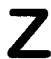
\includegraphics[keepaspectratio]{images/part001_5bbbde23.jpg}}

Note that this is not so in condition (i): a completely secant sequence for A is not necessarily A-regular (exerc. 1).

\begin{enumerate}
\def\labelenumi{\arabic{enumi})}
\setcounter{enumi}{1}
\tightlist
\item
  Let A be a ring, J a finitely generated ideal of A, and p a prime ideal of A containing J. By cor. 2 of th. 1 of § 1, no. 3, we have

\[
\operatorname{prof} _ {A _ {\mathfrak {p}}} (J _ {\mathfrak {p}}; A _ {\mathfrak {p}}) \leqslant [ \kappa (\mathfrak {p}) \otimes_ {A} J: \kappa (\mathfrak {p}) ],
\]

and there is equality if and only if J is completely secant at p.
\end{enumerate}

Suppose that J is distinct from A and generated by a completely secant sequence \((x_{1},\ldots,x_{r})\) . Then we have (prop. 4 of § 1, no. 3, and prop. 1 above)

\[
\operatorname{prof} _ {A} (J; A) = \inf _ {\mathfrak {p} \in V (J)} \operatorname{prof} _ {A _ {\mathfrak {p}}} (J _ {\mathfrak {p}}; A _ {\mathfrak {p}}) = r.
\]

If moreover A is Noetherian, we have \(\operatorname{codim}(\mathrm{V}(\mathrm{J}),\operatorname{Spec}(\mathrm{A}))\leqslant r\) (VIII, § 3, no. 3, prop. 4) and \(\operatorname{prof}_{\mathrm{A}}(\mathrm{J};\mathrm{A})\leqslant \operatorname{codim}(\mathrm{V}(\mathrm{J}),\operatorname{Spec}(\Lambda))\) (§ 1, no. 7, prop. 12), whence finally

\[
\operatorname{prof} _ {\mathrm{A}} (\mathrm{J}; \mathrm{A}) = r = \operatorname{codim} (\mathrm{V} (\mathrm{J}), \operatorname{Spec} (\mathrm{A})) = \operatorname{ht} (\mathrm{J}).
\]

\subsection{Characterization of completely secant ideals}

Let A be a ring and J an ideal of A. The graded A-module \(\bigoplus_{n\in\mathbf{N}}J^{n}\) has a natural structure of graded A-algebra, deduced from the multiplication in the ring A; the identity map of J into \(J^{1}\) therefore extends to a surjective homomorphism of graded A-algebras, said to be canonical

\[
\alpha_ {J}: \mathsf {S} _ {A} (J) \longrightarrow \bigoplus_ {n \in N} J ^ {n}.
\]

By extension of scalars to the ring A/J, from \(\alpha_{\mathrm{J}}\) one deduces a surjective homomorphism of graded A/J-algebras, also said to be canonical

\[
\beta_ {J}: \mathsf {S} _ {\mathrm{A} / J} (\mathrm{J} / \mathrm{J} ^ {2}) \longrightarrow \operatorname{gr} _ {J} (\mathrm{A}),
\]

\(\operatorname{avec} \mathrm{gr}_{\mathrm{J}}(\mathrm{A}) = \bigoplus_{n \in \mathbf{N}} \mathrm{J}^n / \mathrm{J}^{n+1}\) .

THEOREM 1.--- Let A be a Noetherian ring and J an ideal of A. The following conditions are equivalent:

\begin{enumerate}
\def\labelenumi{(\roman{enumi})}
\item
  the ideal J is completely secant ;
\item
  the ideal J is completely secant at every maximal ideal \(\mathfrak{m} \in V(J)\) ;
\item
  the A/J-module J/J² is projective and the canonical homomorphism \(\alpha_{J}: S_{\Lambda}(J) \longrightarrow \bigoplus_{n \in \mathbb{N}} J^{n}\) is bijective;
\item
  the \(\Lambda/\mathrm{J}\) -module \(\mathrm{J}/\mathrm{J}^2\) is projective and the canonical homomorphism \(\beta_{\mathrm{J}}:\mathbf{S}_{\mathrm{A}/\mathrm{J}}(\mathrm{J}/\mathrm{J}^2)\longrightarrow\mathrm{gr}_{\mathrm{J}}(\mathrm{A})\) is bijective.
\end{enumerate}

(i)⇒(ii): this is trivial.

(ii)⇒(iii): suppose condition (ii) is satisfied. It suffices to prove that for every maximal ideal m of A, the \(A_{m}/J_{m}\) -module \(J_{m}/J_{m}^{2}\) is free and the homomorphism \(\alpha_{J_{m}}: S_{A_{m}}(J_{m}) \longrightarrow \bigoplus_{n} J_{m}^{n}\) is bijective (II, § 5, no. 2, th. 1 and § 3, no. 3, th. 1). But these assertions are trivial when m does not belong to V(J), since then we have \(J_{m} = A_{m}\) and they follow from A, X, p.~160, th. 1 and p.~161, remark, when m belongs to V(J).

\begin{enumerate}
\def\labelenumi{(\roman{enumi})}
\setcounter{enumi}{2}
\tightlist
\item
  \(\Rightarrow\) (iv): this is clear.
\end{enumerate}

\((\mathrm{iv}) \Rightarrow (\mathrm{i})\): Suppose condition (iv) is satisfied; let \(\mathfrak{p}\) be a prime ideal of A containing J. Then the \(A_{\mathfrak{p}} / J_{\mathfrak{p}}\) -module \(J_{\mathfrak{p}} / J_{\mathfrak{p}}^2\) is free. Let \(\mathbf{x} = (x_1, \ldots, x_r)\) be a sequence of elements of \(J_{\mathfrak{p}}\) lifting a basis of \(J_{\mathfrak{p}} / J_{\mathfrak{p}}^2\) . The sequence \(\mathbf{x}\) generate \(J_{\mathfrak{p}}\) (Nakayama's lemma), and satisfies by construction condition (iv) of prop. 1. Consequently the ideal \(J_{\mathfrak{p}}\) of \(A_{\mathfrak{p}}\) is completely secant, and J is completely secant at \(\mathfrak{p}\) .

Remark 1. Suppose the ideal J is completely secant; let \((x_1, \ldots, x_r)\) be a sequence of elements of J, such that for every maximal ideal \(\mathfrak{m} \in V(J)\) the canonical images of the \(x_i\) in J/mJ form a basis of this A/m-vector space. Then the A/J-module \(J/J^2\) is free and the canonical images in \(J/J^2\) of the \(x_i\) form a basis of it: it suffices indeed to verify that the images of the \(x_i\) form a basis of the \(A_{\mathfrak{m}}/J_{\mathfrak{m}}\) -module \(J_{\mathfrak{m}}/J_{\mathfrak{m}}^2\) for every \(\mathfrak{m} \in V(J)\) (II, § 3, n° 3, th. 1), which follows from loc. cit., n° 2, prop. 5 and cor. 2, since the \(A_{\mathfrak{m}}/J_{\mathfrak{m}}\) -module \(J_{\mathfrak{m}}/J_{\mathfrak{m}}^2\) is projective (th. 1).

COROLLARY 1.--- Let \(\widehat{\mathrm{A}}\) the separated completion of A for the J-adic topology and \(\widehat{\mathrm{J}} = \mathrm{J}\widehat{\mathrm{A}}\) the separated completion of J. For the ideal \(\widehat{\mathrm{J}}\) of \(\widehat{\mathrm{A}}\) to be completely secant, it is necessary and sufficient that the ideal J of A be completely secant.

Indeed, the canonical map \(\mathrm{gr}_{\mathrm{J}}(\mathsf{A}) \to \mathrm{gr}_{\widehat{\mathrm{J}}}(\widehat{\mathsf{A}})\) is an isomorphism of graded rings; it therefore suffices to apply criterion (iv).

More generally:

COROLLARY 2.--- Let ρ : A → B be a homomorphism of Noetherian rings making B a flat A-module, and let J be an ideal of A.

\begin{enumerate}
\def\labelenumi{\alph{enumi})}
\item
  If J is completely secant, the ideal JB of B is completely secant.
\item
  Suppose that the ideal JB of B is completely secant and that every maximal ideal \(\mathfrak{m} \in \mathrm{V}(\mathrm{J})\) is the inverse image of a maximal ideal of B. Then the ideal J is completely secant. This is the case for example if B is a faithfully flat A-module.
\end{enumerate}

First, note that since the B is a flat A-module, \(J^n \otimes_A B\) is identified with \(J^n B\) and \((J^n / J^{n+1}) \otimes_{A/J} (B/JB)\) is identified with \(J^n B / J^{n+1} B\) for every integer \(n \geqslant 0\) . Assertion a) then follows from criterion (iii). Under the hypotheses of b), the A/J-module B/JB is faithfully flat (I, § 2, no. 7, cor. 2 of prop. 8 and § 3, no. 5, prop. 9) and J is completely secant according to criterion (iv), taking into account I, § 3, no. 1, prop. 2 and no. 6, prop. 12. The last assertion follows from prop. 8 of I, § 3, no. 5.

COROLLARY 3.-- Let A be a Noetherian ring and J a completely secant ideal of A. If A is a Macaulay ring (resp. a Gorenstein ring), then so is A/J.

Indeed, let m be a maximal ideal of A containing J. The ideal \(J_{m}\) of \(\Lambda_{m}\) is generated by a sequence \(A_{m}\) -regular; therefore \((A/J)_{m}\) is a Macaulay ring (resp. a Gorenstein ring) by Example 6 of § 2, No. 5 (resp. Example 2 of § 3, No. 9).

Remark 2. — A Noetherian ring A is said to be a complete intersection ring if, for every maximal ideal m of A, the complete local ring \(\widehat{A_{m}}\) is isomorphic to the quotient of a regular complete local Noetherian ring by a complete intersection ideal. It follows from cor. 3 above and cor. 2 of prop. 12 of § 3, no. 8 that such a ring is a Gorenstein ring.

\subsection{Complete intersection ideals and regular rings}

PROPOSITION 2.--- Let A be a Noetherian ring. The following conditions are equivalent:

\begin{enumerate}
\def\labelenumi{(\roman{enumi})}
\item
  A is regular;
\item
  every maximal ideal of A is completely secant;
\item
  Every ideal J of A such that A/J is regular is completely secant.
\end{enumerate}

(i)⇒(iii): suppose the ring A is regular; let J be an ideal of A such that Λ/J is regular, and let p be a prime ideal of A containing J. Then the local rings \(A_{p}\) and \(A_{p}/J_{p}\) are regular, hence \(J_{p}\) is generated by a completely secant sequence for \(A_{p}\) (VIII, § 5, no. 3, cor. 2 and prop. 2), which means that J is completely secant at p.

\begin{enumerate}
\def\labelenumi{(\roman{enumi})}
\setcounter{enumi}{2}
\tightlist
\item
  (ii): This is clear since a field is a regular ring.
\end{enumerate}

(ii)⇒(i): let m be a maximal ideal of A; under hypothesis (ii), the maximal ideal mA \(_{m}\) of Λ \(_{m}\) is generated by a completely secant sequence for A \(_{m}\) therefore Λ \(_{m}\) is regular (VIII, § 5, no. 2, th. 1). Consequently, A is regular.

PROPOSITION 3.--- Let A be a Noetherian ring and J an ideal of A such that A/J is regular. The following conditions are equivalent:

\begin{enumerate}
\def\labelenumi{(\roman{enumi})}
\item
  the ideal J is completely secant ;
\item
  for every prime (resp. maximal) ideal p of A containing J, the ring A \(_{p}\) is regular;
\item
  The separated completion of A with respect to the J-adic topology is regular.
\end{enumerate}

By th. 1, condition (i) means that for every prime (resp. maximal) ideal p of A containing J, the ideal \(J_{p}\) of the local ring \(A_{p}\) is generated by a completely secant sequence for \(A_{p}\) . Since \(A_{p}/J_{p}\) is regular by hypothesis; this latter condition is equivalent to the fact that \(A_{p}\) let it be regular (VIII, § 5, no. 3, prop. 2 and its cor. 2); this proves the equivalence of (i) and (ii). The equivalence of (ii) and (iii) follows from § 4, no. 2, cor. 3 of prop. 4.

PROPOSITION 4.--- Let A be a regular ring, J an ideal of A and \(A_{0}\) a subring of A such that the canonical homomorphism \(A_{0} \rightarrow A/J\) let it be bijective.

\begin{enumerate}
\def\labelenumi{\alph{enumi})}
\item
  The ideal J is completely secant, the \(A_{0}\) -module \(J/J^{2}\) is projective of finite type, and the ring \(A_{0}\) is regular.
\item
  Let \(\varphi: J/J^{2} \to J\) a section \(A_{0}\) -linear of the canonical surjection \(J \to J/J^{2}\) . The homomorphism of \(A_{0}\) -algebras \(\mathsf{S}_{A_{0}}(J/J^{2}) \longrightarrow A\) extending \(\varphi\) extends to an isomorphism of the completion of the graded ring \(\mathsf{S}_{A_{0}}(J/J^{2})\) on the separated completion of \(A\) for the topology \(J\) -adic.
\end{enumerate}

\begin{enumerate}
\def\labelenumi{\alph{enumi})}
\item
  Let \(\mathfrak{p}\) a prime ideal of A containing J. We have \(\mathfrak{p} = (\mathfrak{p} \cap A_0) \oplus J\) and consequently \(\mathfrak{p}^2 = (\mathfrak{p} \cap A_0)^2 \oplus \mathfrak{p}J\) , hence \(\mathfrak{p}^2 \cap J = \mathfrak{p}J\) . Let \(i\) the canonical injection of \(J\) in \(\mathfrak{p}\) . By what precedes, the map \(i \otimes 1_{A/p}: J \otimes_A A/p \longrightarrow \mathfrak{p} \otimes_A A/p\) is injective, and the same is true of \(i_{\mathfrak{p}} \otimes 1_{\kappa(\mathfrak{p})}: J_{\mathfrak{p}} \otimes_{A_{\mathfrak{p}}} \kappa(\mathfrak{p}) \longrightarrow \mathfrak{p}A_{\mathfrak{p}} \otimes_{A_{\mathfrak{p}}} \kappa(\mathfrak{p})\) . Nakayama's lemma implies that the ideal \(J_{\mathfrak{p}}\) of \(A_{\mathfrak{p}}\) is generated by a subset of a system of coordinates of the regular local ring \(A_{\mathfrak{p}}\) . According to prop. 2 of VIII, § 5, no. 3, the ring \(A_{\mathfrak{p}}/J_{\mathfrak{p}}\) is regular and the ideal \(J_{\mathfrak{p}}\) is completely secant. Thus \(J\) is completely secant, the ring \(A_0\) , isomorphic to \(A/J\) is regular, and the \(A_0\) -module \(J/J^2\) is projective of finite type by th. 1 (no. 2).
\item
  It follows from Thm. 1 that the canonical homomorphism \(\beta_{\mathrm{J}}: \mathsf{S}_{\mathrm{A}_{0}}(\mathrm{J}/\mathrm{J}^{2}) \longrightarrow \mathrm{gr}_{\mathrm{J}}(\mathrm{A})\) is bijective. Let \(f: \mathsf{S}_{\mathrm{A}_{0}}(\mathrm{J}/\mathrm{J}^{2}) \longrightarrow \mathrm{A}\) the homomorphism of \(\mathrm{A}_{0}\) -algebras extending the map \(\mathrm{A}_{0}\) -linear \(\varphi: \mathrm{J}/\mathrm{J}^{2} \longrightarrow \mathrm{J}\) . If A is endowed with the J-adic filtration and \(\mathsf{S}_{\mathrm{A}_{0}}(\mathrm{J}/\mathrm{J}^{2})\) with the filtration associated with its grading, \(\beta_{\mathrm{J}}\) is identified with the homomorphism deduced from \(f\) by passing to the associated graded objects. Assertion b) then follows from III, § 2, no. 8, cor. 3 of th. 1.
\end{enumerate}

\subsection{Graded regular rings}

Let \(A_{0}\) a ring and P a \(A_{0}\) graded module of type N with degrees \textgreater{} 0. Let A denote the ring. \(\mathsf{S}_{\mathrm{A}_{0}}(\mathrm{P})\) ; there exists on A a unique N-grading for which \(A_{0}\) is of degree 0 and P is a sub- \(A_{0}\) -graded module over A. Denote \(A_{+}\) the ideal \(\bigoplus_{n>0} A_{n}\) of A. Then the canonical map \(P \longrightarrow A_{+}/A_{+}^{2}\) is an isomorphism of \(A_{0}\) -graded modules (cf. A, III, p. 76, prop. 10).

If the \(A_{0}\) If the module P is graded free (A, II, p.~167, remark 3) and if \((x_{i})_{i\in I}\) is a basis of P consisting of homogeneous elements, the \(A_{0}\) -graded algebra \(\mathbf{S}_{\Lambda_{0}}(\mathbf{P})\) is isomorphic to the polynomial algebra \(\mathrm{A}_{0}[(\mathrm{X}_{i})_{i\in I}]\) equipped with the graduation for which each \(X_{i}\) is homogeneous of degree \(\deg(x_{i})\) We call \(A_{0}\) -graded polynomial algebra all \(A_{0}\) -graded algebra of type N, isomorphic to a \(A_{0}\) -graded algebra of the preceding form.

When the ring \(\Lambda_0\) is regular and the \(\mathrm{A}_0\) -module P is finitely generated projective, the ring \(\mathsf{S}_{\mathrm{A}_0}(\mathrm{P})\) is regular ( \(\S 4\) (see n° 2, cor. 4 of prop. 4). Conversely:

THEOREM 2.--- Let A be a regular ring, graded of type N. The ring A₀ formed by the elements of degree 0 in A is regular; there exists a finitely generated graded projective A₀-module P with degrees \textgreater{} 0 such that A is isomorphic as a graded A₀-algebra to \(S_{A_{0}}(P)\).

Let P denote the \(A_{0}\) graded module \(A_{+}/A_{+}^{2}\) . By prop. 4 of no. 3, the ring \(A_{0}\) is regular and the \(A_{0}\) -module P is projective and finitely generated. The homogeneous components of P are therefore projective, and there exists a section \(A_{0}\) -linear \(\varphi: P \to A_{+}\) , graded of degree 0, of the canonical surjection \(A_{+} \to P\) . Let \(f: S_{\mathrm{A}_{0}}(\mathrm{P}) \longrightarrow \Lambda\) the homomorphism of \(A_{0}\) -algebras which extends \(\varphi\) . By prop. 4, f extends to an isomorphism of the separated completion of \(\mathbf{S}_{\mathrm{A}_{0}}(\mathrm{P})\) for the topology \(\mathbf{S}_{\mathrm{A}_{0}}(\mathrm{P})_{+}\) -adically onto the separated completion of A for the topology \(A_{+}\) -adic. Consequently, f is injective and its image is dense in A for the topology \(A_{+}\) -adic. But since the induced topologies on the homogeneous components of A are discrete and the image of f is a graded submodule, this implies that f is bijective.

COROLLARY 1. - Let B be a regular ring, graded with positive degrees. Suppose that every \(\mathbf{B}_0\) -module projective of finite type is free.

\begin{enumerate}
\def\labelenumi{\alph{enumi})}
\item
  The ring B \(_{0}\) is integral and regular, and the B \(_{0}\) -algebra 13 is a B \(_{0}\) graduated polynomial algebra, of finite type.
\item
  Let A be a graded subring of B such that \(A_{0} = B_{0}\) and let B be a finitely generated A-module. The following conditions are equivalent:
  \begin{enumerate}
  \def\labelenumii{(\roman{enumii})}
  \item
  the A-module B is graded free;
  \item
  the A-module B is flat;
  \item
  A is a \(A_{0}\) graduated polynomial algebra, of finite type.
  \end{enumerate}
\end{enumerate}

By theorem 2, the ring B₀ is regular, hence a product of regular integral domains (§ 4, no. 2, example 2). For every idempotent element e of B₀, the B₀-module B₀e is projective, hence free, which implies e = 0 or 1; thus B₀ is an integral domain. Assertion a) then follows from theorem 2 and from the fact that a graded projective B₀-module of finite type is graded free.

Let us prove b).

\begin{enumerate}
\def\labelenumi{(\roman{enumi})}
\item
  \(\Leftrightarrow\) (ii): the \(A_0\) -graded flat modules of finite type are graded free (II, § 5, no. 2, cor. 2 of th. 1). The equivalence of (i) and (ii) therefore follows from A, X, p.~144, prop. 8.
\item
  \(\Leftrightarrow\) (iii): since B is integral over A and is a finitely generated A \(_0\) -algebra, A is an A \(_0\) -algebra of finite type (V, § 1, no. 9, lemma 5), hence a Noetherian ring. The equivalence of (ii) and (iii) then follows from the corollary of prop. 8 of § 4, no. 5 and from a) applied to A.
\end{enumerate}

COROLLARY 2.- Let \(k\) be a field, B a \(k\) -graded polynomial algebra, of finite type, and A a graded subalgebra of B. The following conditions are equivalent:

\begin{enumerate}
\def\labelenumi{(\roman{enumi})}
\item
  B is a graded free Λ-module;
\item
  B is a flat A-module;
\item
  ; we have \(\mathrm{Tor}_1^\Lambda (k,\mathbf{B}) = 0\) ;
\item
  the algebra A is a finitely generated graded polynomial k-algebra, and every algebraically free generating sequence of A consisting of homogeneous elements is B-regular.
\end{enumerate}

The implications (i) \(\Rightarrow\) (ii) and (ii) \(\Rightarrow\) (iii) are clear, and implication (iii) \(\Rightarrow\) (i) follows from \(\Lambda\) , X, p.~144, prop. 8, a).

(i)⇒(iv): since the ring B is regular and faithfully flat over A, the ring A is Noetherian by Prop. 11 of I, § 3, No. 6, and regular by Prop. 8 of § 4, No. 5, hence is a graded polynomial k-algebra (Cor. 1, a)). Every algebraically free generating sequence of A is A-regular (A, X, p. 158, example), hence B-regular since B is flat over A.

((iv) \(\Rightarrow\) (iii)): Suppose condition (iv) is satisfied, and let x be an algebraically free generating sequence of A consisting of homogeneous elements. Since the sequence x is A-regular, it is completely secant for A (A, X, p.~157, prop. 5), so that the A-module \(\mathrm{Tor}_{1}^{\mathrm{A}}(k,\mathrm{B})\) is isomorphic to \(\mathrm{H}_{1}(\mathbf{x},\mathrm{B})\) (A, X, p.~159, remark 3); but the latter is zero, since the sequence x is B-regular.

Corollaries 1 and 2 imply Lemma 5 of LIE, V, § 5, No. 5.

\subsection{Regular sequences and scalar extension}

PROPOSITION 5.--- Let \(\mathfrak{p}: A \to B\) a local homomorphism of Noetherian local rings, N a finitely generated B-module, \(\mathbf{x} = (x_1, \ldots, x_r)\) be a sequence of elements of \(\mathfrak{m}_B\) and \(u: A[T_1, \ldots, T_r] \longrightarrow B\) the unique homomorphism of A-algebras such that \(u(T_i) = x_i\) for \(i = 1, \ldots, r\) The following conditions are equivalent:

\begin{enumerate}
\def\labelenumi{(\roman{enumi})}
\item
  the homomorphism u makes N an A{[}T \(_{1}\) ,\ldots{} ,T \(_{r}\) {]}-module flat ;
\item
  the A-module N is flat and, for every A-module M, the sequence x is M ⊗A N-regular;
\item
  the A-module N is flat and the sequence x is \(\kappa_{A} \otimes_{A} N\)-regular ;
\item
  the A-module N/(x₁N + \ldots{} + xᵣN) is flat and the sequence x is N-regular.
\end{enumerate}

(i)⇒(ii): set \(\mathbf{T} = (\mathrm{T}_{1}, \ldots, \mathrm{T}_{r})\) Suppose that the A{[}T{]}-module N is flat. Since A{[}T{]} is flat over A, the A-module N is flat (I, § 2, no. 7, cor. 3 of prop. 8). Let M be an A-module. The sequence T is evidently M{[}T{]}-regular, hence M{[}T{]} ⊗\_\{A{[}T{]}\} N-regular, since N is flat over A{[}T{]}Now the A{[}T{]}-module M{[}T{]} ⊗\_\{A{[}T{]}\} N is identified with M ⊗\_\{A\} N, the homothety of ratio T\_i corresponding to the endomorphism 1\_M ⊗ (x\_i)\_N. Condition (ii) is therefore satisfied.

\begin{enumerate}
\def\labelenumi{(\roman{enumi})}
\setcounter{enumi}{1}
\tightlist
\item
  \(\Rightarrow\) (iii): this is trivial.
\end{enumerate}

(iii)⇒(iv): this follows from prop. 10 of § 1, no. 6.

(iv)⇒(i): let t denote the ideal of A{[}T{]} generated by T. The (A{[}T{]}/t)-module N/tN is flat by hypothesis, and N is ideally separated for t (III, § 5, no. 4, prop. 2). To prove that N is flat over A{[}T{]}, it suffices to prove, in view of th. 1 of loc. cit., no. 2, that the A-module \(\operatorname{Tor}_{1}^{A{[}T{]}}(A{[}T{]}/t,N)\) is zero. But since the sequence T is A{[}T{]}-regular, this module is isomorphic to \(\mathrm{H}_{1}(T,N)\) (A, X, p.~159, remark 3), which is zero since the sequence T is N-regular (loc. cit., p.~157, prop. 5).

COROLLARY. Let \(k\) a field, \(\Lambda\) an \(k\) -local Noetherian algebra, \(\mathbf{x} = (x_1, \ldots, x_r)\) be a sequence of elements of \(\mathfrak{m}_{\mathrm{A}}\) and M a \(\Lambda\) finite type module. Let \(\widehat{\mathrm{A}}\) and \(\widehat{\mathrm{M}}\) the completions of A and M for their topology ( \(x_1\mathrm{A} + \ldots + x_r\mathrm{A}\) -adic; denote by \(u: k[\mathrm{T}_1, \ldots, \mathrm{T}_r] \longrightarrow \mathrm{A}\) the unique homomorphism of \(k\) -algebras such that \(u(\mathrm{T}_i) = x_i\) for \(i = 1, \ldots, r\) , and by \(\hat{u}: k[[\mathrm{T}_1, \ldots, \mathrm{T}_r]] \longrightarrow \widehat{\mathrm{A}}\) the unique continuous homomorphism extending it. The following conditions are equivalent:

\begin{enumerate}
\def\labelenumi{(\roman{enumi})}
\item
  the sequence x is M-regular;
\item
  the homomorphism u makes M into a \(k[T_{1},\ldots,T_{r}]\) -module flat ;
\item
  the homomorphism \(\hat{u}\) makes \(\hat{M}\) a \(k[[T_{1},\ldots,T_{r}]]\) -module flat.
\end{enumerate}

The equivalence of (i) and (ii) follows from the equivalence of conditions (i) and (iv) of Prop. 5; the equivalence of (ii) and (iii) follows from III, § 5, no. 4, Prop. 4.

These results make it possible to characterize Macaulay modules in two important cases. Let us denote \(\Lambda\) a Noetherian local ring, M a finitely generated A-module. It is equivalent to say that the \(\Lambda\) -module M is Macaulay or that the \(\widehat{A}\) -module \(\widehat{M}\) is Macaulay \(\S\) 2, no. 7, cor. 4 of prop. 8). We shall henceforth assume that the Noetherian local ring A is complete.

\begin{enumerate}
\def\labelenumi{\arabic{enumi})}
\tightlist
\item
  Suppose first that A has a subfield; it then admits a field of representatives. \(k\) (IX, § 3, no. 3, th. 1). Let \((x_{1},\ldots ,x_{r})\) a maximal secant sequence for M; denote \(u:k[[\mathrm{T}_{1},\dots ,\mathrm{T}_{r}]]\longrightarrow \Lambda\) the unique continuous homomorphism such that \(u(\mathrm{T}_i) = x_i\) for \(i = 1,\dots ,r\) By lemma 4 b) of IX, § 2, no. 5 and remark 1 of VIII, § 3, no. 2, A/Ann(M) is a \(k[[\mathrm{T}_{1},\dots ,\mathrm{T}_{r}]]\) -module of finite type and consequently M is a \(k[[\mathrm{T}_{1},\dots ,\mathrm{T}_{r}]]\) -finite type module. That said, the following conditions are equivalent:
  \begin{enumerate}
  \def\labelenumii{(\roman{enumii})}
  \item
  the \(k[[\mathrm{T}_1,\dots ,\mathrm{T}_r]]\) -module M is free;
\item
  the A-module M is Macaulay.
\end{enumerate}

Indeed, it is equivalent to say that M is a Macaulay A-module or that the sequence \((x_{1},\ldots,x_{r})\) is M-regular (§ 2, no. 3, th. 1). By the above corollary, this latter condition means that \(k[[T_{1},\ldots,T_{r}]]\) the module M is flat, or equivalently that it is free since it is finitely generated.

\item
  Suppose that the residue field \(\kappa_{\Lambda}\) of A be of characteristic \(p > 0\) and that we have \(\dim(M/pM) < \dim(M)\) . Let \((x_1, \ldots, x_r)\) a maximal secant sequence for M/pM, so that \((p1_{\mathrm{A}}, x_1, \ldots, x_r)\) is a maximal secant sequence for M. Let C be a \(p\) -ring of length \(+\infty\) with residue field \(\kappa_{\Lambda}\) (IX, § 2, no. 3, prop. 5). There exists a homomorphism \(u_0\) from C into A which induces the identity on the residue fields; let \(u: \mathrm{C}[[\mathrm{T}_1, \ldots, \mathrm{T}_r]] \longrightarrow \mathrm{A}\) the unique homomorphism extending \(u_0\) and mapping \(\mathrm{T}_i\) on \(x_i\) for every \(i\) It follows as before from loc. cit., no. 5, lemma 4 that \(u\) makes M a \(\mathrm{C}[[\mathrm{T}_1, \ldots, \mathrm{T}_r]]\) -module of finite type. The following conditions are equivalent:
  \begin{enumerate}
  \def\labelenumii{(\roman{enumii})}
\item
  the C{[}{[}T1, \ldots, Tr{]}{]}-module M is free;
\item
  the A-module M is Macaulay.
\end{enumerate}

Indeed, condition (ii) is equivalent to saying that the sequence \((x_{1},\ldots,x_{r})\) is M-regular and that the homothety with ratio p in \(\mathrm{M}/(x_{1}\mathrm{M}+\ldots+x_{r}\mathrm{M})\) is injective (§ 2, no. 3, th. 1). But this latter condition means that the C-module \(\mathrm{M}/(x_{1}\mathrm{M}+\ldots+x_{r}\mathrm{M})\) is torsion-free, hence flat (Λ, X, p.~9, example 7). Thus, in view of prop. 5, (iv)⇔(i), condition (ii) is equivalent to the fact that the \(C[T_{1},\ldots,T_{r}]\) that the module M is flat, or equivalently (III, § 5, no. 4, prop. 4) that the \(C[[T_{1},\ldots,T_{r}]]\) -module M is flat, that is, free since it is finitely generated.

\end{enumerate}

\subsection{Complete intersection ideals and extension of scalars}

PROPOSITION 6. - Let \(\rho: A \to B\) a homomorphism of Noetherian rings and J an ideal of B. The following conditions are equivalent:

\begin{enumerate}
\def\labelenumi{(\roman{enumi})}
\item
  the A-module B/J is flat and the ideal J is completely secant.
\item
  for every \(\mathfrak{q} \in \mathrm{V}(\mathrm{J})\) , the A-module \(\mathrm{B}_{\mathfrak{q}}\) is flat and, for every A-algebra \(\mathrm{A}'\) such that the ring \(\Lambda' \otimes_{\mathrm{A}} \mathrm{B}\) noetherian ring, the ideal \(\mathrm{J}(\mathrm{A}' \otimes_{\mathrm{A}} \mathrm{B})\) of \(\mathrm{A}' \otimes_{\mathrm{A}} \mathrm{B}\) is completely secant;
\item
  for every maximal ideal n of B containing J, the A-module \(B_{n}\) is flat and the ideal \(\mathrm{J}(\kappa(\rho^{-1}(\mathfrak{n}))\otimes_{\mathrm{A}}\mathrm{B}_{\mathfrak{n}})\) of \(\kappa(\rho^{-1}(\mathfrak{n}))\otimes_{\mathrm{A}}\mathrm{B}_{\mathfrak{n}}\) is completely secant.
\end{enumerate}

By th. 1 of no. 2, condition (i) is equivalent to condition (i′) (resp. (i′\,The following:

(i') (resp. (i'\,for every prime (resp. maximal) ideal q of B containing J, the \(A_{p^{-1}(q)^{-}}\) -module \(B_{q}/J_{q}\) is flat and the ideal \(J_{q}\) of \(B_{q}\) is generated by a sequence \(B_{q}\) -regular.

\((i') \Rightarrow (ii)\) : suppose \((i')\) verified. Let \(A'\) an A-algebra such that the ring \(B' = A' \otimes_A B\) let it be Noetherian. Let \(q\) be a prime ideal of B containing \(J\) ; set \(p = \rho^{-1}(q)\) . Since \(B_q'\) is identified with \(A_p' \otimes_{A_p} B_q\) , it follows from the implication \((iv) \Rightarrow (ii)\) of prop. 5 ( \(n^o 5\) ) that the ideal \(JB_q'\) of \(B_q'\) is generated by a sequence \(B_q'\) -regular and that \(B_q\) is flat over \(A_p\) , hence on \(A\) . Moreover, for every prime ideal \(r\) of \(B'\) containing \(JB'\) , the inverse image \(q\) of \(r\) in B contains \(J\) and \(B_r'\) identifies with a ring of fractions of \(B_q'\) Thus \(JB_r'\) is a completely secant ideal of \(B_r'\) and \(JB'\) is a completely secant ideal of \(B'\) .

\begin{enumerate}
\def\labelenumi{(\roman{enumi})}
\setcounter{enumi}{1}
\tightlist
\item
  \(\Rightarrow\) (iii): this is trivial.
\end{enumerate}

(iii)⇒ (i'\,): assume (iii) holds. Let n be a maximal ideal of B containing J; set m = ρ \(^{-1}\) (n). Let x be a sequence of elements of Jn whose images in Jn/nJn form a basis of this κ(n)-vector space. The sequence x generates Jn; by prop. 1 of no. 1, it is (κ(m) ⊗A Bn)-regular. Since the Am-module Bn is flat by hypothesis, it follows from the implication (iii)⇒ (iv) of prop. 5 that condition (i'\,') is satisfied.

Remark 1.--- Suppose that the equivalent conditions of prop. 6 are satisfied. Since B/J is flat over A, for every A-algebra A', the canonical sequence of A'-modules

\[
0 \rightarrow \Lambda^ {\prime} \otimes_ {A} J \longrightarrow A ^ {\prime} \otimes_ {A} B \longrightarrow A ^ {\prime} \otimes_ {A} (B / J) \rightarrow 0
\]

is therefore exact, and the canonical homomorphism \(A'\otimes_A J \longrightarrow J(A'\otimes_A B)\) is bijective.

\section{Extension of scalars in regular algebras}

\subsection{Essentially finitely generated algebras}

Let \(k\) a ring. Let A be an \(k\) -algebra and \(\mathbf{x} = (x_i)_{i \in I}\) a family of elements of A; denote by \(\mathbf{A}'\) the subalgebra of A generated by the \(x_i\) . We say that \(\mathbf{x}\) is an essentially generating family of the \(k\) -algebra A if, for every element \(a\) of A, there exists an element \(s\) of \(\mathbf{A}'\) , invertible in A, such that \(sa\) belong to \(\mathbf{A}'\) . This is equivalent to saying that, for every \(a \in \mathbf{A}\) , there exist polynomials P and Q in \(k[(\mathrm{X}_i)_{i \in I}]\) such that \(\mathrm{Q}(\mathbf{x})\) is invertible in A and that one has \(a = \mathrm{P}(\mathbf{x})\mathrm{Q}(\mathbf{x})^{-1}\) .

We shall say that a \(k\) -algebra A is essentially of finite type if it admits a finite essentially generating family. This is equivalent to saying that there exists a \(k\) -algebra A' of finite type and a multiplicative subset S of A' such that the \(k\) -algebra A is isomorphic to \(\mathrm{S}^{-1}\mathrm{A}'\) .

Examples.--- 1) Saying that an extension L of a field K is an essentially finitely generated K-algebra means that it is a finitely generated extension in the sense of A, V, p.~11, def. 2. The K-algebra L is of finite type only if it is a finite-degree extension of K (V, § 3, no. 4, cor. 3 of th. 3).

\begin{enumerate}
\def\labelenumi{\arabic{enumi})}
\setcounter{enumi}{1}
\tightlist
\item
  For a \(k\) -algebra to be local and essentially of finite type, it is necessary and sufficient that it be isomorphic to a \(k\) -algebra of the form \(\mathsf{A}_{\mathfrak{p}}\) , where A is a \(k\) finitely generated algebra and \(\mathfrak{p}\) a prime ideal of A (cf.~II, § 2, no. 5, prop. 11 (iii)).
\end{enumerate}

PROPOSITION 1. - If the ring k is Noetherian, every essentially finitely generated k-algebra is a Noetherian ring.

This follows from III, § 2, no. 10, cor. 3 of th. 2 and II, § 2, no. 4, cor. 2 of prop. 10.

From the definition, we deduce the following properties:

PROPOSITION 2.--- a) Every quotient algebra of a k-algebra essentially of finite type is essentially of finite type.

\begin{enumerate}
\def\labelenumi{\alph{enumi})}
\setcounter{enumi}{1}
\item
  Every ring of fractions of an essentially finitely generated k-algebra is an essentially finitely generated k-algebra.
\item
  The \(k\) -algebra product of a finite family of \(k\) -algebras essentially of finite type is essentially of finite type.
\item
  Let \(k \to k'\) a ring homomorphism; for every \(k\) -algebra A essentially of finite type, the \(k'\) -algebra \(A_{(k')} = k' \otimes_k \Lambda\) is essentially of finite type.
\end{enumerate}

COROLLARY.- Let A be an \(k\) -algebra essentially of finite type and B a \(k\) -algebra that is Noetherian. Then the ring \(\mathrm{A} \otimes_k \mathrm{B}\) is Noetherian.

Indeed, it is a B-algebra essentially of finite type (prop. 2, d)) and one applies proposition 1.

PROPOSITION 3. Let \(k\) a ring, A a linearly topologized formally smooth \(k\) -algebra and B an A-algebra. If A is essentially of finite type over \(k\) and B essentially of finite type over A, then B is essentially of finite type over \(k\) .

Let \(\rho: A \to B\) the canonical map. Let \(x = (x_i)_{i \in I}\) a finite essentially generating family of the \(k\) -algebra \(A\) and \(A'\) the subalgebra it generates; let \(y = (y_j)_{j \in J}\) a finite essentially generating family of the \(A\) -algebra \(B\) . Let \(B'\) the sub- \(k\) -algebra of \(B\) generated by the \(\rho(x_i)\) and the \(y_j\) . Let \(b \in B\) ; by hypothesis there exist polynomials \(P\) and \(Q\) in \(A[(Y_j)_{j \in J}]\) such that \(Q(y)\) let it be invertible in \(B\) and that we have \(Q(y)b = P(y)\) The nonzero coefficients of \(P\) and \(Q\) are finite in number; there exists a polynomial \(R \in k[(X_i)_{i \in I}]\) such that \(R(x)\) let it be invertible in \(A\) and that \(R(x)P\) and \(R(x)Q\) belong to \(A'[[(Y_j)_{j \in J}]\) Then \(\rho(R(x))Q(y)\) be invertible in \(B\) and one has

\[
\rho (\mathrm{R} (\mathbf {x})) \mathrm{Q} (\mathbf {y}) b = \rho (\mathrm{R} (\mathbf {x})) \mathrm{P} (\mathbf {y}) \in \mathrm{B} ^ {\prime}.
\]

Thus the elements \(\rho(x_i)\) for \(i \in I\) and \(y_j\) for \(j \in J\) form an essentially finitely generating family of the \(k\) -algebra B.

COROLLARY. -- The tensor product of two k-algebras essentially of finite type is a k-algebra essentially of finite type.

Indeed, let A and B be two essentially finitely generated k-algebras. Then \(A \otimes_{k} B\) is essentially of finite type over A (prop. 2, d)) hence over k (prop. 3).

\subsection{Tensor products of Macaulay or Gorenstein algebras}

PROPOSITION 4. Let k be a field, A an essentially finitely generated k-algebra, and B a k-algebra.

\begin{enumerate}
\def\labelenumi{\alph{enumi})}
\item
  If A and B are Macaulay rings, then so is A ⊗k B.
\item
  If A and B are Gorenstein rings, then so is \(\Lambda\otimes_{k}\mathrm{B}\) .
\end{enumerate}

Suppose that A and B are Macaulay (resp. Gorenstein) rings, and let us prove that the same is true of \(A \otimes_{k} B\) . The ring \(A \otimes_{k} B\) is noetherian (no. 1, cor. of prop. 2). The A-module \(A \otimes_{k} B\) is free, hence flat. By prop. 10 of § 2, no. 7 (resp. cor. 1 of prop. 12 of § 3, no. 8), it suffices for us to prove that \(\kappa(\mathfrak{p}) \otimes_{k} B\) is a Macaulay ring (resp. Gorenstein ring) for every prime ideal p of A. The extension \(\kappa(\mathfrak{p})\) Since k is of finite type (no. 1, prop. 2 and example 1), we are therefore reduced to proving the statement in the case where the k-algebra A is a finitely generated extension K of k.

Let \((t_{1},\ldots,t_{n})\) a transcendence basis of K over k, so that K is a finite degree extension of the pure extension \(k^{\prime}=k(t_{1},\ldots,t_{n})\) (A, V, p.~112, prop. 17). The ring \(B^{\prime}=k^{\prime}\otimes_{k}B\) is isomorphic to a ring of fractions of the polynomial ring \(B[T_{1},\ldots,T_{n}]\) therefore is a Macaulay (resp. Gorenstein) ring by cor. 2 of prop. 10 of § 2, no. 7 (resp. cor. 3 of prop. 12 of § 3, no. 8). Since \(K\otimes_{k}B\) is identified with \(K\otimes_{k^{\prime}}B^{\prime}\) we are reduced to proving assertions a) and b) when K is a finite-degree extension of k.

The ring K ⊗k B is then a free B-module of finite rank, hence a Macaulay B-module. By § 2, no. 6, cor. 1 of prop. 8, it is a Macaulay ring, which proves a). Suppose now that B is a Gorenstein ring. There exist subextensions K \(_{i}\) with 0 ≤ i ≤ m, of K

\[
k = \mathrm{K} _ {0} \subset \mathrm{K} _ {1} \subset \dots \subset \mathrm{K} _ {m} = \mathrm{K}
\]

such that \(K_{i}\) let a \(K_{i-1}\) -monogenic algebra for \(i = 1, \ldots, m\) , and this allows us to reduce to the case where the extension K of k is monogenic (of finite degree). The canonical homomorphism \(B \to K \otimes_{k} B\) makes \(K \otimes_{k} B\) a flat B-algebra and, for every \(\mathfrak{q} \in \operatorname{Spec}(B)\) , the ring \((\mathrm{K} \otimes_{k} \mathrm{B}) \otimes_{\mathrm{B}} \mathfrak{k}(\mathfrak{q})\) , isomorphic to \(K \otimes_{k} \mathfrak{k}(\mathfrak{q})\) , is a \(\mathfrak{k}(\mathfrak{q})\) -monogenic algebra, hence a Gorenstein ring (§ 3, n° 9, example 5). Thus \(K \otimes_{k} B\) is a Gorenstein ring (§ 3, n° 8, cor. 1 of prop. 12), which completes the proof of b).

COROLLARY 1.--- Let \(k\) a field, K an extension of \(k\) and \(\Lambda\) an \(k\) -algebra essentially of finite type. For \(\mathrm{A}_{(\mathrm{K})}\) to be a Macaulay ring (resp. Gorenstein ring), it is necessary and sufficient that the same hold for A.

If A is a Macaulay (resp. Gorenstein) ring, then so is \(\mathrm{A}_{(\mathrm{K})}\) By prop. 4. Since \(\mathrm{A}_{(\mathrm{K})}\) is a faithfully flat A-module, the converse follows from prop. 10 of § 2, no. 7 (resp. from cor. 1 of prop. 12 of § 3, no. 8).

COROLLARY 2.--- Let k be a Noetherian ring, and let A and B be k-algebras. Assume that A is flat and essentially of finite type over k. If A and B are Macaulay rings (resp. Gorenstein rings), then A ⊗k B is a Macaulay ring (resp. Gorenstein ring).

Suppose first that B is a field; denote \(\varphi\) the canonical homomorphism from \(k\) into B, and \(\mathfrak{r}\) its kernel. The homomorphism \(\varphi\) induces a homomorphism from the field of fractions \(\kappa(\mathfrak{r})\) of \(k/\mathfrak{r}\) into B. Then A \(\otimes_{k}\) B is identified with (A \(\otimes_{k}\) K(r)) \(\otimes_{\kappa(\mathfrak{r})}\) B; as \(\varphi^{-1}(0)=\mathfrak{r}\) the ring A \(\otimes_{k}\) K(r) is a Macaulay (resp. Gorenstein) ring by prop. 10 of § 2, no. 7 (resp. cor. 1 of prop. 12 of § 3, no. 8). The assertion follows in this case from cor. 1.

Let us pass to the general case. The B-algebra A⊗ \(_{k}\) B is flat, and noetherian by the cor. of prop. 2 of no. 1. For each prime ideal q of B, the ring (A⊗ \(_{k}\) B)⊗ \(_{B}\) κ(q), which is identified with A⊗ \(_{k}\) κ(q) is a Macaulay (resp. Gorenstein) ring by the preceding results. One concludes by applying prop. 10 of § 2, no. 7 (resp. cor. 1 of prop. 12 of § 3, no. 8).

\subsection{\texorpdfstring{Separable extension of the base field in regular algebras \(^{1}\) or normal}{Separable extension of the base field in regular or normal algebras (1)}}
\footnotetext[1]{In this section, an algebra over a field \(k\) is called regular if it is a regular ring. In particular, every extension of \(k\) is a regular algebra. This notion should not be confused with that of a regular extension, introduced in A, V, p. 135, Definition 2, which will not be used here.}

Lemma 1.--- Let A be a Noetherian ring, the union of an increasing filtered family \((\mathrm{A}_{\alpha})_{\alpha\in\mathbb{I}}\) of Noetherian subrings.

\begin{enumerate}
\def\labelenumi{\alph{enumi})}
\item
  If the rings \(\Lambda_{\alpha}\) are regular and if A is a \(\mathrm{A}_{\alpha}\) -module flat for all \(\alpha \in \mathrm{I}\) the ring A is regular.
\item
  If the rings \(\mathrm{A}_{\alpha}\) are normal (§ 1, no. 8), A is normal.
\end{enumerate}

\begin{enumerate}
\def\labelenumi{\alph{enumi})}
\item
  Let \(\mathfrak{m}\) a maximal ideal of A; for every \(\alpha \in I\) let us denote \(\mathfrak{m}_{\alpha}\) the ideal \(\mathfrak{m} \cap A_{\alpha}\) of \(A_{\alpha}\) . Since A is Noetherian, \(\mathfrak{m}\) is of finite type and there exists an element \(\alpha\) of I such that \(\mathfrak{m} = A\mathfrak{m}_{\alpha}\) so that the A-module \((A_{\alpha}/\mathfrak{m}_{\alpha}) \otimes_{A_{\alpha}} A\) is isomorphic to \(A/m\) Since A is flat over \(A_{\alpha}\) , one has \(\mathrm{dp}_{A}(A/m) \leqslant \mathrm{dp}_{A_{\alpha}}(A_{\alpha}/\mathfrak{m}_{\alpha})\) (A, X, p.~141, lcmc 2). Since the rings \(A_{\alpha}\) are regular, it follows that A is regular \(\S 4\) (no. 2, prop. 4).
\item
  Since the \(A_{\alpha}\) are reduced, A is reduced. Let a and b be elements of A such that b is not a zero divisor and the element a/b of the total ring of fractions of A is integral over \(\Lambda\) . There exists a monic polynomial \(P \in A[X]\) such that \(P(a/b) = 0\) . Let \(\alpha\) an element of I such that the ring \(A_{\alpha}\) contains a, b, and the coefficients of P. Since \(A_{\alpha}\) is normal, there exists \(c \in A_{\alpha}\) such that a = bc. Thus a/b = c belongs to \(\Lambda\) and \(\Lambda\) is normal.
\end{enumerate}

Lemma 2. -- Let \(k\) a field, K and L extensions of \(k\) Suppose that K is of finite type and that one of the extensions K or L is separable. Then the ring \(\mathrm{K} \otimes_{k} \mathrm{L}\) is regular.

Let A denote the ring K ⊗k L; it is Noetherian by the corollary of Prop. 2 (no. 2). Suppose first that the extension K is separable. By A, V, p.~130, corollary, there exists a transcendence basis t = (t₁, \ldots..., tₙ) of K such that K is a finite separable extension of the pure extension k(t). The ring E = k(t) ⊗k L, isomorphic to a ring of fractions of a polynomial ring over L, is regular (§ 4, n° 2, cor. 5 of prop. 4); for every prime ideal p of E, the ring κ(p) ⊗E A is isomorphic to κ(p) ⊗k(t) K, hence to a finite product of fields (A, V, p.~35, def. 1, p.~34, th. 4, and p.~33, prop. 5). Since A is a free E-module, it is a regular ring by the cor. of prop. 9 of § 4, n° 5.

Suppose now that L is separable over k. By the first part of the proof, the ring \(K \otimes_{k} L'\) is regular for every finitely generated subextension \(L'\) of L. We conclude by applying Lemma 1.

PROPOSITION 5.--- Let k be a field, A a k-algebra, and K an extension of k. Suppose that A is essentially of finite type or that the extension K is of finite type.

\begin{enumerate}
\def\labelenumi{\alph{enumi})}
\item
  If the ring A \(_{(K)}\) is regular (resp. normal), the ring A is regular (resp. normal).
\item
  If the ring \(\Lambda\) is regular (resp. normal) and if the extension K of \(k\) is separable, the ring \(\mathrm{A}_{(\mathrm{K})}\) is regular (resp. normal).
\end{enumerate}

The A-module \(A_{(K)}\) is free, hence faithfully flat; assertion a) therefore follows from the corollary of Prop. 8 in I, § 3, No. 5 and from Prop. 8 of § 4, No. 5 (resp. from Cor. 2 of Th. 4 of § 1, No. 10). Under the hypotheses of b), for every prime ideal p of A, the ring \(\kappa(\mathfrak{p})\otimes_{k}K\) is regular (lemma 2), and a fortiori normal (§ 4, no. 2, cor. 2 of prop. 4). Assertion b) therefore follows from the corollary of prop. 9 of § 4, no. 5 (resp. from cor. 3 of th. 4 of § 1, no. 10).
